\documentclass[11pt]{article}
\usepackage{times,url}
\usepackage{code} 
%\usepackage{proof}
%\usepackage{newcode}
%\usepackage{epsfig}
\usepackage{xcolor}
\usepackage{graphicx}
\usepackage{epstopdf} 

\newcommand{\Para}[1]{{\vspace{0.03in}\noindent \bf {#1}}}


\newcommand{\cut}[1]{}

\newcommand{\appref}[1]{Appendix~\ref{#1}}
\newcommand{\secref}[1]{Section~\ref{#1}}
\newcommand{\tblref}[1]{Table~\ref{#1}}
\newcommand{\figref}[1]{Figure~\ref{#1}}
\newcommand{\listingref}[1]{Listing~\ref{#1}}
%\newcommand{\pref}[1]{{page~\pageref{#1}}}

\newcommand{\eg}{{\em e.g.}}
\newcommand{\cf}{{\em cf.}}
\newcommand{\ie}{{\em i.e.}}
\newcommand{\etc}{{\em etc.\/}}
\newcommand{\naive}{na\"{\i}ve}
\newcommand{\role}{r\^{o}le}
\newcommand{\forte}{{fort\'{e}\/}}
\newcommand{\appr}{\~{}}

\newcommand{\bftt}[1]{{\ttfamily\bfseries{}#1}}
\newcommand{\kw}[1]{\bftt {#1}}
\newcommand{\Pthen}{\kw{Pthen}}
\newcommand{\pads}{\textsc{pads}}
\newcommand{\padsl}{\textsc{padsl}}
\newcommand{\padst}{\textsc{pads/t}}
\newcommand{\datatype}{\textsc{PADS/T}}
%\newcommand{\datatype}{\textsc{DataType}}
\newcommand{\C}{\textsc{C}}
\newcommand{\perl}{\textsc{Perl}}
\newcommand{\ml}{\textsc{ml}}
\newcommand{\sml}{\textsc{sml}}
\newcommand{\smlnj}{\textsc{sml/nj}}
\newcommand{\java}{\textsc{java}}
\newcommand{\ddl}{\textsc{ddl}}
\newcommand{\xml}{\textsc{xml}}
\newcommand{\datascript}{\textsc{DataScript}}
\newcommand{\packettypes}{\textsc{PacketTypes}}
\newcommand{\erlang}{\textsc{Erlang}}

\newcommand{\Core}{Ad hoc}
\newcommand{\core}{ad hoc}
\newcommand{\pvalue}{\core{} value}
\newcommand{\ppat}{\core{} pattern}
\newcommand{\ptype}{\core{} type}

\newcommand{\padsc}{\textsc{pads}/\C{}}
\newcommand{\padsml}{\textsc{pads}/\ml{}}

\newcommand{\dibbler}{Sirius}
\newcommand{\ningaui}{Altair}
\newcommand{\darkstar}{Regulus}

\newcommand{\pdgood}{{\tt G}}
\newcommand{\pdbad}{{\tt B}}
\newcommand{\pdnest}{{\tt N}}
\newcommand{\pdsem}{{\tt S}}
\newcommand{\ptypes}{T}
\newcommand{\patreadpd}[2]{{\tt #1<<#2>>}}
\newcommand{\btm}{\cd{BOT}}


\newcommand{\lsem}{{[\![}}
\newcommand{\rsem}{{]\!]}}


\newcommand{\figHeight}[4]{\begin{figure}[tb]
	\centerline{
	            \epsfig{file=#1,height=#4}}
	\caption{#2}
	\label{#3}
	\end{figure}}

%% Environment for typesetting BNF grammars. Uses display math mode.
\newenvironment{bnf}
     {%% local command definitions:
        %% BNF definition symbol
      \def\->{\rightarrow}
%%      \def\::={{::=} &}
      \def\::={\bnfdef &}
      \def\|{\bnfalt}
      \newcommand{\name}[1]{\text{##1}}
        %% non-terminal
      \newcommand{\nont}[1]{{##1}}
      \newcommand{\meta}[1]{& ##1 &}
      \newcommand{\descr}[1]{& \text{// ##1}}
      \newcommand{\opt}[1]{ [##1] }
      \newcommand{\opnon}[1]{\opt{\nont{##1}}}
      \newcommand{\none}{\epsilon}
      \newcommand{\nwln}{\\ &&&}
      \newcommand{\nlalt}{\\ && \| &}
      \[\begin{array}{lrlll}
     }
     {\end{array}\]}

\newcommand{\mcd}[1]{\mathtt{#1}}
\newcommand{\ppair}[3]{#1{:}#2 \mathrel{**} #3}
\newcommand{\parray}[3]{#1\;\mcd{Parray}(#2,#3)}
\newcommand{\pset}[3]{\{#1{:}#2\,|\,#3\}}
\newcommand{\pstream}[1]{#1\;\mcd{stream}}
\newcommand{\precord}[1]{\{\{#1\}\}}


%%%%%%%%%%%%%%%%%%%%%%%%%%%%%%%%%%%%%%%%%%%%%%%%%%%%%%%%%%%%%%%%%%%%%%%%%%%%
\voffset             0in    %  top vertical offset
\hoffset             0in    %  left horizontal offset
\oddsidemargin       0pt    %  Left margin on odd-numbered pages.
\evensidemargin      0pt    %  Left margin on even-numbered pages.
\topmargin           0pt    %  Nominal distance from top of page to top of
\headheight          0pt    %  Height of box containing running head.
\headsep             0pt    %  Space between running head and text.
\textwidth         6.5in    %  Width of text on page
\textheight          9in    %  Height of text on page
\setlength{\parskip}{.05in}
\renewcommand{\floatpagefraction}{.9}
\renewcommand{\textfraction}{0.1}
\renewcommand{\baselinestretch}{1.01}
%\input{macro}  %%%  other macro definitions

%%%%%%%%%%%%%%%%%%%%%%%%%%%%%%%%%%%%%%%%%%%%%%%%%%%%%%%%%%%%%%%%%%%%%%%%%%%%
\begin{document}
\setcounter{page}{1}
\pagenumbering{roman}
\appendix
%%%%%%%%%%%%%%%%%%%%%%%%%%%%%%%%%%%%%%%%%%%%%%%%%%%%%%%%%%%%%%%%%%%%%%%%%%%%
\section{SHF:Small:Language Support for Ad Hoc Data Processing}
%%%%%%%
%%%%%%%%%%%%%%%%%%%%%%%%%%%%%%
% \centerline{
% \begin{tabular}{cc}
%           \\[-1ex]
% \multicolumn{2}{c}{Automatic Tool Generation for Ad Hoc Scientific Data} \\
%           & \\[-1ex]
% David Walker (PI)\\
% Princeton University\\[2ex]
% \end{tabular}}
%%%%%%%%%%%%%%%%%%%%%%%%%%%%%%

\paragraph*{Intellectual Merits:} 
In every scientific discipline, researchers are digitizing their knowledge and
beginning to use computational methods to categorize,
query, filter, search, diagnose, and visualize their data.  
While this effort is leading to remarkable advances,
it is also generating enormous amounts of {\em ad hoc data}.
Ad hoc data is any data for which standard data processing tools
such as query engines, statistical packages, graphing tools, parsers, printers,
transformers or programming libraries are not readily available.
This data, which is often unpredictable, poorly documented,
filled with errors, high volume and unwieldy,
poses tremendous challenges to its users and the software
that manipulates it.  We cannot maximize the productivity of top 
computational scientists unless we can maximize the efficiency and 
accuracy with which they deal with this data.

Our overall goal is to alleviate the burden, risk and confusion
associated with ad hoc data.  Our overall strategy is (1) to develop a
specification language capable of precisely describing any ad hoc data
format at an easy-to-understand, high level of abstraction and (2) to
automatically generate useful data processing tools including
programming libraries, a query engine, format converters, a
statistical summarizer, a histogram generator and others.
 
We will accomplish our task by building upon our preliminary data
description and processing system, \pads{}, created by the PI and his
collaborators.  This preliminary system demonstrates the basic
feasibility of the \pads{} approach, but there is much research to do.
While the work to date demonstrates the feasibility of the \pads{}
approach, the \pads{} design and implementation are still in their
infancy: We have discovered many common, real-world data formats that
the current PADS infrastructure is incapable of describing, parsing or
analyzing.  To address these deficiencies, we propose to explore
innovative ways of extending the basic \pads{} specification language
and related infrastructure.  The second thrust of our research
involves improving the automatic tool generation infrastructure in the
\pads{} system.  The current tool generation system is brittle,
inflexible and suffers from subpar performance.  We will develop a
novel extension to \pads{} that allows users to augment \pads{}
descriptions with application-specific attributes and customizations.
The attributes convey semantic information to the tool generators and
the customizations improve error-handling and performance.  Our new
architecture has the promise of being substantially more robust,
flexible and efficient.  Finally, in order to improve the reliability
of the infrastructure, we will formalize \pads{} and prove important
correctness properties of our formal model.  Overall, this proposal
involves challenging research in language design, efficient systems
implementation and semantic analysis, all aimed at solving real-world
data processing problems.

\paragraph*{Broader Impacts:}  We are collaborating with Kathleen Fisher
and Mary Fernandez at
AT\&T who will be able to use our tools to address real problems such
as telephone fraud detection.  In addition, our tools will be freely
available to researchers and scientists over the web.  Moreover, part
of our mission will be to work with specific biologists and
physicists at Princeton and the broader community to help them with
their data processing needs.  We have already been meeting with Olga
Troyanskaya, who works in Princeton's Lewis-Sigler Institute for
Integrative Genomics on pathway modeling and analysis of
protein-protein interactions, and with Rachel Mandelbaum, Ph.D. candidate
in physics who analyzes cosmology data.  Many of our proposed extensions to
\pads{} were inspired directly by their data processing needs.  

The collaboration between Computer Science and Genomics will also be an
excellent platform for developing interdisciplinary undergraduate
research projects.  The PI has a proven track-record 
for following through with undergraduate and graduate
educational plans:  Last year, his undergraduate student advisee, Rob Simmons,
won the Princeton Computer Science Senior Thesis Award;
last year and the year before he organized two NSF-sponsored summer schools
on secure and reliable computing.


\newpage
% %%%%%%%%%%%%%%%%%%%%%%%%%%%%%%%%%%%%%%%%%%%%%%%%%%%%%%%%%%%%%%%%%%%%%%%%%%%%
% \section{Table of Contents}
% \tableofcontents\
% \vspace*{.1in} 
% \begin{center}
% {\Large\bf\em{}This is a place-holder. Fastlane generates this page automatically.}
% \end{center} 
% \newpage
%%%%%%%%%%%%%%%%%%%%%%%%%%%%%%%%%%%%%%%%%%%%%%%%%%%%%%%%%%%%%%%%%%%%%%%%%%%%
\pagenumbering{arabic}
\setcounter{page}{1}
%%%%%%%%%%%%%%%%%%%%%%%%%%%%%%%%%%%%%%%%%%%%%%%%%%%%%%%%%%%%%%%%%%%%%%%%%%%%
\section{Project Description}

\subsection{Introduction}
\label{ssec:intro}

An {\em ad hoc data format} is any nonstandard data format for which
parsing, querying, analysis or transformation tools are not readily
available.  \xml{} is not an ad hoc data format --- there are hundreds
of tools for reading, querying, and transforming \xml{}.  However,
network administrators,
data analysts, computer scientists,
biologists, chemists, and physicists deal with ad hoc
data in a myriad of complex formats on a daily basis.
This data, which is often unpredictable, poorly documented,
and filled with errors
poses tremendous challenges to its users and the software
that manipulates it.  
Our goal is to alleviate the burden, risk and confusion associated
with ad hoc data by developing a universal data processing system
capable of 
concisely and accurately describing any ad hoc data source at an 
easy-to-understand, high-level of abstraction, and
automatically generating a suite of highly reliable and
efficient data processing tools that make understanding, manipulating 
and transforming ad hoc data an effortless task.
%\end{enumerate}

Together with Kathleen Fisher (Senior Personnel),
his collaborators and students, the PI has developed 
a system called \pads{} (Processing Ad hoc Data Sources)~\cite{padsweb,fisher+:pads,fisher+:popl06,mandelbaum+:pads-ml,fisher+:dirttoshovels} that 
helps to address some of these concerns.
It includes a high-level, declarative language for describing
ad hoc data formats and it is possible to generate tools for
parsing, printing, querying, generating histograms and 
statistical summaries of data, and transforming 
data into \xml.  An online demo~\cite{padsdemo} illustrates
our progress to date.  However, the PI's work date has generated
important new scientific questions and shown the need for new language
support and tool generation technology.  In particular, if funded, the 
PI will pursue the following critical new research agenda:


\begin{enumerate}
\item {\bf Language support for multi-level directory systems.}
Many ad hoc data sets are physically represented as collections of 
data files, organized in a multi-level directory system.
The PI will develop powerful, new extensions to PADS that allow programmers
to specify the structure of these multi-level directory systems
and generate libraries for programming against them.
\item {\bf Semi-automatic data description generation.}
While using the PADS data description language speeds the generation
and maintainance of data processing tools, a user must invest some effort
to learn the language syntax and semantics.  The PI will simplify
and improve the process of writing descriptions by developing 
an entirely new kind of {\em text mark-up language} that 
allows users to add simple
labels to raw data sources, and from such labels, generate full descriptions.
Such descriptions can, in turn, serve as lasting documentation or be 
used %processed by the pads compiler
to generate useful programming tools.
\item {\bf Grammatical foundations and efficient implementation.}  
Many complex, modern text and binary data formats require a very rich collection
of features in order to describe them declaratively:  
{\em full context-free grammars}, the ability to bind 
parts of a data source to {\em variables} for later use in
{\em constraints}, {\em parameters} on non-terminals and the
ability to include pre-defined libraries as {\em black boxes} 
within a description.  The PI will develop a new grammatical 
theory that explains how to implement this rich collection of features
efficiently.  
\item {\bf Automatic generation of new data processing tools.} 
The PI will use the newly developed theory and implementation techniques 
to build important new tools including description-directed 
data generators for use in testing data processing infrastructure
and a multi-source, ad hoc data query engine.
\end{enumerate}


%% \begin{enumerate}
%% \item {\bf Language support for multi-level directory systems.}
%% Many ad hoc data sets are physically represented as collections of 
%% data files, organized in a multi-level directory system.
%% The PI will develop powerful, new extensions to PADS that allow programmers
%% to specify the structure of these multi-level directory systems
%% and to develop new tool-generation infrastructure capable of
%% automatically producing useful tools for monitoring, querying and programming
%% against these complex data sources.
%% \item {\bf Semi-automatic data description generation.}
%% While using the PADS data description language speeds the generation
%% and maintainance of data processing tools, a user must invest some effort
%% to learn the language syntax and semantics.  The PI will develop 
%% an entirely new kind of {\em text mark-up language} that allows users to add simple
%% labels to raw data sources, and from such labels, generate full descriptions
%% that can in turn serve as lasting documentation or be used to generate useful
%% programming tools.
%% \item {\bf Grammatical foundations and efficient implementation.}  
%% Many complex, modern text and binary data formats require a very rich collection
%% of features in order to describe them declaratively:  
%% {\em full context-free grammars}, the ability to bind 
%% parts of a data source to {\em variables} for later use in
%% {\em constraints}, {\em parameters} on non-terminals and the
%% ability to include pre-defined libraries as {\em black boxes} 
%% within a description.  The PI will develop a new grammatical 
%% theory that explains how to implement this rich collection of features
%% efficiently.  In addition, the PI will use the new theory to build
%% important new tools including a random data generator for using
%% in testing data processing infrastructure.
%% \end{enumerate}

Overall, our research combines novel language design, high-performance
systems engineering and theoretical analysis.  It will substantially
increase the overall productivity of data analysts, researchers and
software architects who deal with ad hoc data regularly, and it will
improve the security and reliability of the software they produce.
Finally, we have the plans and the corporate connections necessary
to transfer our technology to industry as well as ideas on how
we can apply our results so as to have a broad impact on research in the
natural sciences, where ad hoc data is pervasive.

The PI and his team are uniquely qualified to carry out this research agenda
and have an unsurpassed track record of top research production
in this important area.  In particular, this research team has produced 
relevant papers in 4 of the last 5 ACM SIGPLAN Conferences on Principles
of Programming Languages (POPL 06~\cite{fisher+:popl06}, 
POPL 07~\cite{mandelbaum+:pads-ml}, POPL 08~\cite{fisher+:dirttoshovels}
and POPL 10~\cite{jim+:data-dependent-grammars})
as well as an article for the Journal of the ACM~\cite{fisher+:700journal} 
--- POPL being widely considered the top conference
in programming language theory and design and the Journal of the
ACM often considered the top journal in computer science. Few other research
projects can boast such a claim.  
In addition to producing a variety of other papers in the area~\cite{fisher+:pads,fernandez+:padx,pads-sigmod06,burke+:cagi07,mandelbaum+:dual-semantics,mandelbaum+:generic-padsml,pads-sigmod08,token-ambiguity,pads:distributed,pads:wasl},
the research team has also 
delivered software free to download on the 
web~\cite{padscdistributions,padsmldistributions,padslearndistributions} 
and has developed on-line demos~\cite{padsdemo} 
so students and researchers can learn about their results and
experiment with their research ideas.

In the rest of this introduction, we will explain the immense
challenges and risks posed by ad hoc data in more detail and
we explain how the \pads{} system we have already
implemented helps handle them.  
Reviewers who are familiar with \pads{} and are already convinced that the ad hoc data processing
problem is both technically challenging and extremely important may want to skim this
section quickly in order to more quickly begin reading about our
proposed research in Section~\ref{sec:research}.  
%Section~\ref{sec:research} ends with a
%brief collaboration plan.  Next, Section~\ref{sec:impacts} explains how we 
will make a broad impact (1) on industry through technology transfer,
(2) on research in the natural sciences and (3) on graduate and
undergraduate education in computer science.  Section~\ref{sec:related} contains
further information on related research and Section~\ref{sec:prior} summarizes the
PI's results from previous NSF awards.

\Para{The Challenges of Ad Hoc Data.}
There are vast amounts of useful data stored in
traditional databases and \xml{} formats, but there is just as much in
ad hoc formats.  \figref{figure:data-sources} provides some information
on ad hoc data formats from several different domains ranging from genomics
to networking to finance to internal corporate billing information.  
They include ASCII, binary, and Cobol data formats, with
both fixed and variable-width records, ranging in size from
relatively small files through network applications which process over
a gigabyte per second.  Common errors include undocumented data,
corrupted data, missing data, and multiple missing-value
representations.


\begin{figure*}
\begin{center}
\begin{tabular}{@{}|l|l|l|l|l|}
\hline
Name: Use                           & Representation    & Processing Problems \\ \hline\hline
Gene Ontology (GO)~\cite{geneontology}:                  & Variable-width    & White-space ambiguities \\
Gene Product Information 	      & ASCII records &  \\ \hline
Web server logs (CLF):                & Fixed-column      & Race conditions on log entry\\ 
Measuring web workloads               & ASCII records     & Unexpected values\\ \hline
AT\&T Call detail data:                          & Fixed-width       & Undocumented data\\
Phone call fraud detection            & binary records  & \\ \hline 
AT\&T billing data:                 & Cobol             &  Unexpected values\\ 
Monitoring billing process          &                   & Corrupted data feeds \\ \hline
Newick:   Immune                    & Fixed-width ASCII records & None \\ 
system response simulation          & in tree-shaped hierarchy &\\ \hline                                
OPRA:                               & Mixed binary \& ASCII records 
                                                       & 100-page informal \\
Options-market transactions         & with data-dependent unions & documentation \\ \hline
Palm PDA:                           & Mixed binary \& character & No high-level  \\
Device synchronization              & with data-dependent constraints & documentation available\\ \hline
\end{tabular}
\caption{Selected ad hoc data sources.}
\label{figure:data-sources}
\end{center}
\end{figure*}


Processing ad hoc data is challenging for a variety of further reasons. 
First, ad hoc data typically arrives ``as is'': the analysts
who receive it can only say ``thank you,'' not request a more
convenient format.  Second, documentation for the format may not exist
at all, or it may be out of date.  A common phenomenon is for a field
in a data source to fall into disuse.  After a while, a new piece of
information becomes interesting, but compatibility issues prevent data
suppliers from modifying the shape of their data, so instead they
hijack the unused field, often failing to update the documentation in
the process.

Third, such data frequently contain errors, for a variety of reasons:
malfunctioning equipment, race conditions on log entry~\cite{wpp},
non-standard values to indicate ``no data available,'' human error in
entering data, unexpected data values, \etc{} The appropriate response
to such errors depends on the application.  Some applications require
the data to be error free: if an error is detected, processing needs
to stop immediately and a human must be alerted.  Other applications
can repair the data, while still others can simply discard erroneous
or unexpected values.  For some applications, errors in the data can
be the most interesting part because they can signal where two systems
are failing to communicate.

% A fourth challenge is that ad hoc data sources can be high volume:
% AT\&T's call-detail stream contains roughly 300~million calls per day
% requiring approximately 7GBs of storage space. Although this data is
% eventually archived in a database, analysts mine it profitably before
% such archiving~\cite{kdd98,kdd99}. More challenging, the \ningaui{}
% project at AT\&T accumulates billing data at a rate of 250-300GB/day,
% with occasional spurts of 750GBs/day. Netflow data arrives from Cisco
% routers at rates over a gigabyte per second~\cite{gigascope}! Such
% volumes mean it must be possible to process the data without loading
% it all into memory at once.

Finally, before anything can be done with an ad hoc data source,
someone has to produce a suitable parser for it.  Today, people tend
to use \C{} or \perl{} for this task.  Unfortunately, writing parsers
this way is tedious and error-prone, complicated by the lack of
documentation, convoluted encodings designed to save space, the need
to produce efficient code, and the need to handle errors robustly to
avoid corrupting down-stream data.  Moreover, the parser writers'
hard-won understanding of the data ends up embedded in parsing code,
making long-term maintenance difficult for the original writers and
sharing the knowledge with others nearly impossible.

\Para{\pads{}:  Taking on the Challenge of Ad Hoc Data.}
The \pads{} system~\cite{padsweb,fisher+:pads,fisher+:popl06,mandelbaum+:pads-ml,fisher+:dirttoshovels} makes life easier for data analysts by addressing
each of the concerns outlined in the previous section.
It provides a declarative data description
language that permits analysts to describe the physical layout of
their data, \textit{as it is}.  The language also permits analysts to
describe expected semantic properties of their data so that deviations can
be flagged as errors. The intent is to allow analysts to capture in a
\pads{} description all that they know about a given data source.
%In exchange
%and to provide the analysts with a library of useful routines in exchange. 


%\pads{} descriptions are intended to be concise enough to serve as
%documentation and flexible enough to describe many ASCII, binary,
%Cobol, and mixed data formats.  In addition, useful software tools
%can be generated from the descriptions and this feature provides
%strong incentive for keeping the descriptions current, allowing them
%to serve as living documentation.  

Given a \pads{} description, the \pads{} compiler produces
customizable \C{}~\cite{fisher+:pads} or O'Caml~\cite{mandelbaum+:pads-ml} 
libraries and tools for parsing, manipulating, and
summarizing the data.  The core libraries include functions for
reading the data, writing it back out in its original form, 
detecting and summarizing errors in the data, iterating over the data, 
writing it into a canonical \xml{} form, pretty printing it in forms suitable for
loading into a relational database, and accumulating statistical
properties.  An auxiliary library provides an instance of the data API
for Galax~\cite{galax,galaxmanual}, an implementation of XQuery.  This
library allows users to query data with a \pads{} description as if
the data were in \xml{} without having to convert to \xml, which often
can avoid an 8-10 times blow-up in space requirements.  

As a high-level, domain-specific language,
\pads{} provides a number of important benefits to
its users.  The generated parsing code checks
all possible error cases: system errors related to the input file,
buffer, or socket; syntax errors related to deviations in the physical
format; and semantic errors in which the data violates user
constraints.  Because these checks appear only in generated code, they
do not clutter the high-level declarative description of the data
source.  Moreover, since tools are generated
automatically by a compiler rather than written by hand, 
they are far more likely to be robust
and far less likely to have dangerous vulnerabilities such as
buffer overflows.  In addition, as formats change and are updated,
one can make a small change in the high-level description
and the compiler will takes care of the rest.  It is extremely unlikely
new vulnerabilities or buffer overflows will be added to the code
base over time as formats change.

The \pads{} system also
addresses performance in a number of ways.  First, we compile the
\pads{} description rather than simply interpret it to reduce run-time
overhead.  Second, the generated parser provides multiple entry
points, so the data consumer can choose the appropriate level of
granularity for reading the data into memory to accommodate arbitrarily large
data sources.  Finally, we parameterize library functions by
\textit{masks}, which allow data analysts to choose which semantic
conditions to check at run-time, permitting them to specify all known
properties in the source description without forcing all users of that
description to pay the run-time cost of checking them.

%% The result of a parse is a pair consisting of a canonical
%% in-memory {\em representation} of the data and a {\em parse descriptor}. 
%% The parse
%% descriptor precisely characterizes both the syntactic and the semantic
%% errors that occurred during parsing.  This structure allows analysts
%% to choose how to respond to errors in application-specific ways.

% With such huge datasets, performance is critical. The \pads{} system
% addresses performance in a number of ways.  First, we compile the
% \pads{} description rather than simply interpret it to reduce run-time
% overhead.  Second, the generated parser provides multiple entry
% points, so the data consumer can choose the appropriate level of
% granularity for reading the data into memory to accommodate very large
% data sources.  Finally, we parameterize library functions by
% \textit{masks}, which allow data analysts to choose which semantic
% conditions to check at run-time, permitting them to specify all known
% properties in the source description without forcing all users of that
% description to pay the run-time cost of checking them.

% Given the importance of the problem, it is perhaps surprising that
% more tools do not exist to solve it.  \xml{} and relational databases
% only help with data already in well-behaved formats.  Lex and Yacc are
% both over- and under- kill.  Overkill because the division into a
% lexer and a context free grammar is not necessary for many ad hoc data
% sources, and under-kill in that such systems require the user to build
% in-memory representations manually, support only ASCII sources, and
% don't provide extra tools.  ASN.1~\cite{asn} and related
% systems~\cite{asdl} allow the user to specify an in-memory
% representation and generate an on-disk format, but this doesn't help
% when given a particular on-disk format.  Existing ad hoc description
% languages~\cite{gpce02,sigcomm00,erlang} are steps in the right
% direction, but they focus on binary, error-free data and they do not
% provide auxiliary tools.

% We propose to extend and improve the current \pads{}\ prototype by engaging
% in three intertwined research efforts:

% \begin{enumerate}
% \item Our experience with real-world data has revealed that
% the current \pads{}\ system is unable to process many common
% data formats.  We propose a number of extensions to \pads{} 
% that will greatly improve its expressive power and enable
% us to handle many more important ad hoc formats.
% \item While \pads{}\ can automatically generate tools for providing
% statistical data summaries, querying ad hoc data and generating
% \xml, the tool generation process is extremely brittle, inflexible
% and results in low-performance software.  We propose to redesign
% the automatic tool generation process using a principled methodology
% based upon a novel \pads{}-attribute system that can communicate
% semantic information across tools.  Our new methodology will
% improve the flexibility and reliability of the \pads{} system.
% \item There is no formal description of the \pads{} language
% and no semantics for the compiler or tools.  We propose to
% formalize the language and analyze the semantics of the
% compiler.  Our formal analysis may find bugs or flaws in the
% \pads{} system and will improve our confidence in the implementation.
% \end{enumerate}

% \noindent
% In addition, part of our mission will be to use \pads{} to provide
% data processing tools for researchers in the natural sciences including
% biology, chemistry and physics.  

% In building the \pads{} system, we faced challenges on two fronts:
% designing the data description language and
% crafting the generated libraries and tools.
% In the rest of the paper, 
% we describe each of these designs.
% We also give examples to show how useful they have been at AT\&T.



% \figref{figure:data-sources} summarizes some of the sources we have
% worked with.  They include ASCII, binary, and Cobol data formats, with
% both fixed and variable-width records, ranging in size from
% relatively small files through network applications which process over
% a gigabyte per second.  Common errors include undocumented data,
% corrupted data, missing data, and multiple missing-value
% representations.


% \subsection{Common Log Format}
% Web servers use the Common Log Format (CLF) to log client
% requests~\cite{wpp}.  Researchers use such logs to measure
% properties of web workloads and to evaluate protocol changes
% by "replaying" the user activity recorded in the log.
% This ASCII format consists of a sequence of
% records, each of which has seven fields: the host name or IP address
% of the client making the request, the account associated with the
% request on the client side, the name the user provided for
% authentication, the time of the request, the actual request, the
% \textsc{http} response code, and the number of bytes returned as a
% result of the request.  The actual request has three parts: the
% request method (\eg, \texttt{GET}, \texttt{PUT}), the requested
% \textsc{uri}, and the protocol version.  In addition, the second and
% third fields are often recorded only as a '-' character to indicate
% the server did not record the actual data.  \figref{figure:clf-records}
% shows a couple of typical records.

\Para{The Current \pads{} Language Infrastructure.}
In order to understand \pads{} further, we
will examine an example of ad hoc data:
a tiny fragment of data from the Gene Ontology Project~\cite{geneontology}.  
Data in this format is widely used by molecular biologists to
analyze gene products produced by various organisms.
\figref{figure:dibbler-records} shows a tiny sample of
the format.  Cursory examination of the example data reveals
first of all that this is an ASCII format with two 
logical parts, a header portion (that portion beginning with
\texttt{format-version} and ending with the first blank line)
and a main portion, which includes a sequence of 
information blocks separated by blank lines (only one such block 
is shown in the example).  The format
designers call these information blocks {\em stanzas}.
Each stanza begins with a stanza tag, which may be either
\texttt{[Term]}, as shown in the example data, or
\texttt{[Typeref]}.  On the following line,
the first element of each stanza, is
the string \texttt{id}, followed by a colon, followed by a
GO identifier.  A GO identifier is the word GO, followed
by another colon, followed by a string.  
After the first mandatory id field, the rest of the stanza includes
any number of identifier, colon, field entries.
% While this format is actually remarkably simple, and
% we have left out several details in this coarse description,
% it should be apparent that English is a poor
% language for describing data formats!

\begin{figure*}
\begin{small}
%\begin{center}
\begin{verbatim}
format-version: 1.0
date: 11:11:2005 14:24
saved-by: midori
auto-generated-by: DAG-Edit 1.419 rev 3
default-namespace: gene_ontology
remark: cvs version: $Revision: 1.3 $
subsetdef: goslim_goa "GOA and proteome slim"
subsetdef: goslim_yeast "Yeast GO slim"
subsetdef: goslim_plant "Plant GO slim"
subsetdef: goslim_generic "Generic GO slim"
subsetdef: gosubset_prok "Prokaryotic GO subset"

[Term]
id: GO:0000001
name: mitochondrion inheritance
namespace: biological_process
def: "The distribution of mitochondria\, including the mitochondrial 
genome\, into daughter cells after mitosis or meiosis\, mediated by 
interactions between mitochondria and the cytoskeleton." [PMID:10873824, 
PMID:11389764, SGD:mcc]
is_a: GO:0048308 ! organelle inheritance
is_a: GO:0048311 ! mitochondrion distribution

\end{verbatim}
\caption{Tiny example of Gene Ontology data. (Some lines broken to
present data on this page.)}
\label{figure:dibbler-records}
%\end{center}
\end{small}
\end{figure*}

Now, we can examine how to use \pads{} to describe 
the {\em physical layout} and 
{\em semantic properties} of our ad hoc data source. 
The language provides a type-based model:
basic types describe atomic data such as integers, characters, 
strings, dates, urls, \etc, while
structured types describe compound data built from simpler pieces.
\suppressfloats

In a bit more detail,
the \pads{} library provides a collection of broadly useful base
types.  Examples include 8-bit unsigned integers (\cd{Puint8}), 32-bit
integers (\cd{Pint32}), dates (\cd{Pdate}), strings (\cd{Pstring}),
and IP addresses (\cd{Pip}).  Semantic conditions for such base types
include checking that the resulting number fits in the indicated
space, \ie, 16-bits for \cd{Pint16}.  By themselves, these base types
do not provide sufficient information to allow parsing because they do
not specify how the data is coded, \ie{}, in ASCII, EBCDIC, or binary.
To resolve this ambiguity, \pads{} uses the \textit{ambient} coding,
which the programmer can set.  By default, \pads{} uses ASCII.  
% To
% specify a particular coding, the description writer can select base
% types which indicate the coding to use.  Examples of such types
% include ASCII 32-bit integers (\cd{Pa_int32}), binary bytes
% (\cd{Pb_int8}), and EBCDIC characters (\cd{Pe_char}).  In addition to
% these types, users can define their own base types to specify more
% specialized forms of atomic data.


\begin{figure}[t]

\begin{code}
/* www.geneontology.org OBO flat file format. */
\mbox{}
#define COLON ':'
\mbox{}
Precord Pstruct OBO\_tag\_value\_pair\{
  Pstring(:COLON:) tag;  
  Pre "/: */"; 
  Pstring\_ME(:Peor:) val;
\};
\mbox{}
int hasTag(OBO\_tag\_value\_pair p,char *tag)\{
  return Pstring\_eq\_cstr(&p.tag,tag); 
\};
\mbox{}
Precord Pstruct OBO\_header\{
  ...
\};
\mbox{}
Penum OBO\_stanza\_type\{ Term, Typeref \};
\mbox{}
Precord Pstruct OBO\_stanza\_tag \{
    '['; OBO\_stanza\_type s\_type; ']';
\};
\mbox{}
Precord Pstruct OBO\_stanza\{
  OBO\_stanza\_tag       tag;
  OBO\_tag\_value\_pair   id      : hasTag(id,"id");
  OBO\_tag\_value\_pair[] tvpairs : Pterm(Peor);
\};
\mbox{}
Psource Pstruct OBO\_file\{
  OBO\_header hdr;
  OBO\_stanza[] stanzas;
\};
\end{code}

%\begin{code}
\kw{Precord} \kw{Pstruct} summary\_header\_t \{
  "0|";
  Puint32       tstamp;
\};
\mbox{}
\kw{Pstruct} no\_ramp\_t \{
  "no\_ii";
  Puint64 id;
\};
\mbox{}
\kw{Punion} dib\_ramp\_t \{
  Pint64     ramp;
  no\_ramp\_t  genRamp;
\};
\mbox{}
\kw{Pstruct} order\_header\_t \{
       Puint32             order\_num;
 '|';  Puint32             att\_order\_num;
 '|';  Puint32             ord\_version;
 '|';  \kw{Popt} pn\_t           service\_tn;
 '|';  \kw{Popt} pn\_t           billing\_tn;
 '|';  \kw{Popt} pn\_t           nlp\_service\_tn;
 '|';  \kw{Popt} pn\_t           nlp\_billing\_tn;
 '|';  \kw{Popt} Pzip           zip\_code;
 '|';  dib\_ramp\_t          ramp;
 '|';  Pstring(:'|':)      order\_type;
 '|';  Puint32             order\_details;
 '|';  Pstring(:'|':)      unused;
 '|';  Pstring(:'|':)      stream;
 '|';
\};
\mbox{}
\kw{Pstruct} event\_t \{
  Pstring(:'|':) state;   '|';
  Puint32        tstamp;
\};
\mbox{}
\kw{Parray} eventSeq \{
  event\_t[] : \kw{Psep}('|') && \kw{Pterm}(\kw{Peor});
\} \kw{Pwhere} \{
  \kw{Pforall} (i \kw{Pin} [0..length-2] :
           (elts[i].tstamp <= elts[i+1].tstamp));
\};
\mbox{}
\kw{Precord} \kw{Pstruct} entry\_t \{
  order\_header\_t  header;
  eventSeq        events;
\};
\mbox{}
\kw{Parray} entries\_t \{
  entry\_t[];
\};
\mbox{}
\kw{Psource} \kw{Pstruct} out\_sum\{
  summary\_header\_t  h;
  entries\_t         es;
\};
\end{code}


\caption{Abbreviated \pads{} description for Gene Ontology data.}
\label{figure:dibbler}
\end{figure}


To describe more complex data, \pads{} provides a collection of
declarations based upon the type structure of the host programming
language (which may either be C or O'Caml, though for the rest of this
section, we assume it is C).  In
particular, \pads{} has \mytt{Pstruct}s, \mytt{Punion}s, and \mytt{Parray}s
to describe record-like structures, alternatives, and sequences,
respectively.  \mytt{Penum}s describe a fixed collection of literals,
while \mytt{Popt}s provide convenient syntax for optional data.  Each of
these types can have an associated predicate that indicates whether a
value calculated from the physical specification is indeed a legal
value for the type.  For example, a predicate might require that two
fields of a \mytt{Pstruct} are related or that the elements of a
sequence are in increasing order.  Programmers can specify such
predicates using \pads{} expressions and functions, written using a
\C{}-like syntax.  Finally, \pads{} \mytt{Ptypedef}s can be used to
define new types that add further constraints to existing types.

\pads{} types can be parameterized by values.  This mechanism serves
both to reduce the number of base types and to permit the format and
properties of later portions of the data to depend upon earlier
portions.  For example, the base type \cd{Puint_FW(:x:)} specifies
an unsigned integer physically represented by exactly \cd{x}
characters, where \cd{x} is a value that has been read earlier in the
parse.  The type \cd{Pstring(:COLON:)} describes a string
terminated by a colon (when \texttt{COLON} is defined to be \texttt{':'}).  
Parameters can be used with compound types like arrays and unions to
specify the size of an array or which branch of a union should be
taken.  This parameterization is what makes PADS a {\em dependently-typed}
language and substantially different from languages based on
context-free grammars or regular expressions.

\figref{figure:dibbler} gives an abbreviated \pads{} description 
for the Gene Ontology
data.  
We will use this example to illustrate some of the basic
features of the current \pads{} language.  
In \pads{} descriptions, types are declared before they are used, 
so the type that describes the totality of the data source appears 
at the bottom of the description.  In this case,
the type \texttt{OBO\_file} describes the the entirety of the
GO data source (the \texttt{Psource} type qualifier indicates
this fact explicitly).  \texttt{OBO\_file} is a \mytt{Pstruct} type with
two fields, a \texttt{hdr} field, with type  \texttt{OBO\_header}
and a \texttt{stanzas} field with type \texttt{OBO\_stanza[]},
an array of \texttt{OBO\_stanza}s of arbitrary length.
In general, \mytt{Pstruct}s describe fixed sequences of data with 
unrelated types.  A little further up the description, there is
a slightly more complex \mytt{Pstruct}:  \texttt{OBO\_stanza\_tag}.
This struct contains two kinds of fields, named fields, like
before, and unnamed fields \texttt{'['} and \texttt{']'}.
These unnamed fields match literal characters in the data, in this
case square brackets.  In 
\texttt{OBO\_tag\_value\_pair}, another unnamed field involving 
a regular expression (introduced by \texttt{Pre}) matches a colon
followed by any number of spaces.  Named fields are included in
the internal representation of the data, while unnamed fields are
not.  

Both \texttt{OBO\_tag\_value\_pair} and
\texttt{OBO\_stanza\_tag} mentioned above are preceded by the
\texttt{Precord} type qualifier.  
The notion of a record varies depending upon the data encoding.  
ASCII data typically uses new-line characters to delimit 
records, binary sources tend to have fixed-width records, while 
COBOL sources usually store the length of each record before the actual data.
\pads{} supports each of these encodings of records and allows users to define
their own encodings.  By default, \pads{} assumes records are new-line terminated.  The constant \texttt{Peor} is also set to this
\texttt{e}nd-\texttt{o}f-\texttt{r}ecord marker, and may be used anywhere in a
description, as we did in the
type \texttt{OBO\_tag\_value\_pair}.
\texttt{Precords} have error-recovery semantics -- if errors 
in the data cause the parser to become seriously confused,
it will attempt to recover to a record boundary.
In practice, we have found this to be a very robust recovery mechanism
for ad hoc data.  

The \texttt{OBO\_stanza} structure 
illustrates the use of some simple semantic constraints.
For instance, following the \texttt{id} field is the constraint
\texttt{hastag(id,"id")}, which is defined earlier in the file
as a function in defined in C.  In general, such constraints should
be pure (have no externally visible effects), but otherwise may be
arbitrary C expressions.  Notice also that the first argument to the constraint
is \texttt{id}, the name of the current field.  More generally,
constraints may refer to any type parameters in scope and any previous field.
The type parameters in particular, allow information concerning data
just parsed to be passed arbitrarily far forward in a description.
The second semantic constraint in \texttt{OBO\_stanza} is
\texttt{Pterm(Peor)}, which is a built-in constraint for 
controlling array termination.  In this case, it states that
the array terminates when it sees an end-of-record marker 
\texttt{Peor} following any array element.  
In general, \pads{} provides a rich collection
of array-termination conditions: reaching a maximum size, finding 
a terminating literal 
or satisfying a user-supplied predicate over the already-parsed portion of 
the \mytt{Parray}.  \pads{} also has convenient syntax for 
specifying separator symbols that
appear between elements of an array and declaring inter-element
constraints including sorting.

%% One last feature of note in this description is the \texttt{Penum}
%% \texttt{OBO\_stanza\_type}.  \texttt{Penum}s specify that
%% the data must be one of several fixed strings, in this case, 
%% either \texttt{Term} or \texttt{Typeref}.  \pads{} also admits
%% \texttt{Punion}s of several forms for more general sorts of alternatives
%% in data formats.

%Other examples of \pads{} descriptions and an online demo may be
%found at \url{www.padsproj.org}.


% Returning to the CLF description in \figref{figure:wsl}, the \mytt{Penum} type \cd{method_t} describes
% a collection of data literals.  During parsing, \pads{} interprets these
% constants using the ambient character encoding.  The \mytt{Ptypedef} 
% \cd{response_t} describes possible server response codes in CLF data by adding
% the constraint that the three-digit integer must be between 100 and 600.

% \setlength{\floatsep}{0pt}
% \setlength{\dblfloatsep}{0pt}
% \setcounter{totalnumber}{4}
% \setcounter{dbltopnumber}{2}
% \begin{figure*}[t!]
% \begin{small}
% \begin{center}
% \begin{code}
% \chapter{Common log format example}
\section{pads description}
\section{c header file}
% \end{code}
% \vskip -2ex
% \caption{Tiny example of web server log data.}
% \label{figure:clf-records}
% \end{center}
% \end{small}
% \end{figure*}


% \begin{figure}
% \begin{code}
\kw{Punion} client\_t \{
  Pip       ip;      /- 135.207.23.32
  Phostname host;    /- www.research.att.com
\};
\mbox{}
\kw{Punion} auth\_id\_t \{
  Pchar unauthorized : unauthorized == '-';
  Pstring(:' ':) id;
\};
\mbox{}
\kw{Pstruct} version\_t \{
  "HTTP/";
  Puint8 major; '.';
  Puint8 minor;
\};
\mbox{}
\kw{Penum} method\_t \{
    GET,    PUT,  POST,  HEAD,
    DELETE, LINK, UNLINK
\};
\mbox{}
bool chkVersion(version\_t v, method\_t m) \{
  \kw{if} ((v.major == 1) && (v.minor == 1)) \kw{return} true;
  \kw{if} ((m == LINK) || (m == UNLINK)) \kw{return} false;
  \kw{return} true;
\};
\mbox{}
\kw{Pstruct} request\_t \{
  '\\"';   method\_t       meth;
  ' ';    Pstring(:' ':) req\_uri;
  ' ';    version\_t      version :
                  chkVersion(version, meth);
  '\\"';
\};
\mbox{}
\kw{Ptypedef} Puint16\_FW(:3:) response\_t :
         response\_t x => \{ 100 <= x && x < 600\};
\mbox{}
\kw{Precord} \kw{Pstruct} entry\_t \{
         client\_t       client;
   ' ';  auth\_id\_t      remoteID;
   ' ';  auth\_id\_t      auth;
   " ["; Pdate(:']':)   date;
   "] "; request\_t      request;
   ' ';  response\_t     response;
   ' ';  Puint32        length;
\};
\mbox{}
\kw{Psource} \kw{Parray} clt\_t \{
  entry\_t [];
\}
\end{code}

% \caption{\pads{} description for web server log data.}
% \label{figure:wsl}
% \end{figure}

\subsection{Overview of Planned Research}
\label{sec:research}

%% Our central research agenda is divided into three broad subsections,
%% which we will discuss here; our broader impacts will be discussed in the next 
%% section.  First, our experience with real-world data has revealed that
%% it is common to find a single logical repository of ad hoc data
%% physically represented as a collection of files, organized in a structured
%% multi-level directory system.  We propose to extend the \pads{}\ 
%% language and tool generation system so that it can describe and
%% process such rich repositories.  Second, while
%% \pads{} lifts the level abstraction for generation of data processing
%% tools, \pads{} takes some time to learn and descriptions take time to
%% write.  We propose to develop an entirely new way to generate \pads{}
%% descriptions, by using of a novel kind of markup language.  This new
%% paradigm holds the promise of making it possible to describe
%% rich, complex data sources in just minutes and then immediately
%% generate data processing tools, all with very little 
%% learning overhead.  Third, we propose to develop new algorithms for
%% parsing and format analysis based on developing a new theory
%% of data-dependent grammars.
%% Overall, our research combines novel language
%% design, high-performance systems engineering and theoretical analysis,
%% all aimed at solving crucial data processing problems.


\begin{figure}
\begin{center}
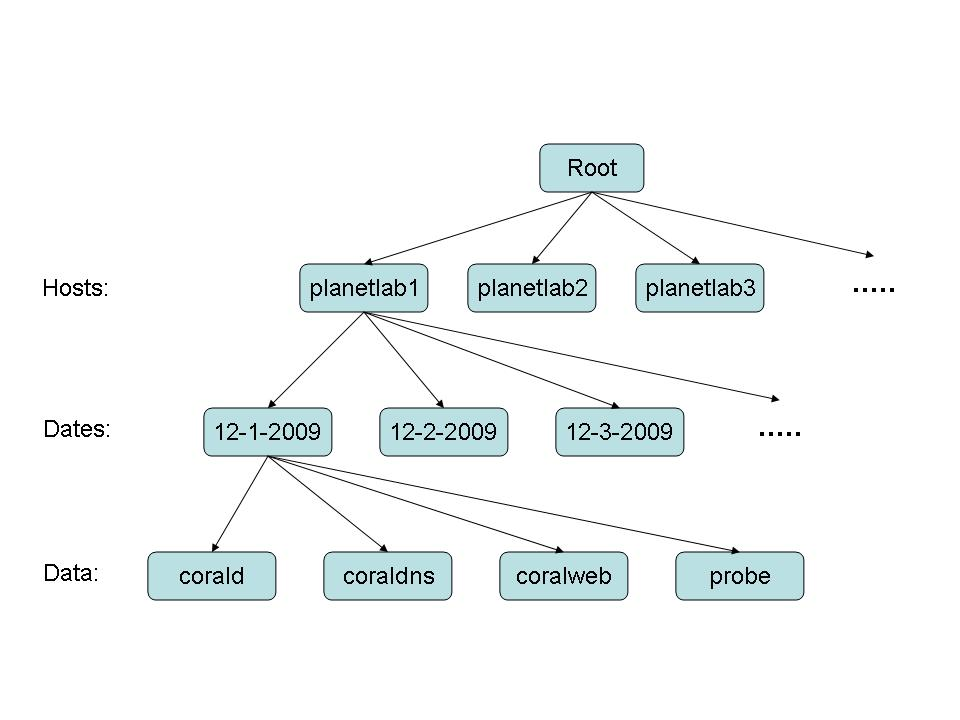
\includegraphics[width=100mm]{coral-pic.jpg}
\end{center}
\vspace{-1.8cm}

\caption{Directory Structure of the Coral Monitoring and Logging Subsystem}
\label{fig:coral-pic}
\end{figure}


\Para{Hierarchical, Multi-source Data Descriptions.}
Often, a single logical data source is represented
as several distinct, concrete repositories.   This is the case
in the GO data source we have examined, where data is split into four disjoint
files: a molecular function file, a biological process file,
a cellular component file and a term definitions file -- only one of 
those files was described in the previous subsection.
However, it is not uncommon for data repositories to, in fact, be much, much 
larger and much more complex.
%the size and number of repositories that make up a single source
%may vary widely.  At the other end of the spectrum are systems involving
%continuous monitoring of widescale phenomena that automatically
%produce new data at phenominal rates.  
As another example, the Coral
content distribution system~\cite{freedman:coral} acts on a completely
different scale.  It
collects log files
from hundreds of servers distributed world-wide on short time scales
and stores them in a hierarchical set of directories
Figure~\ref{fig:coral-pic} shows how this complex ad hoc information
system is organized.  The Figure shows that 
a top-level root directory contains a set of subdirectories,
one per remote host in the Coral system.  Each of those subdirectories contains
contains a further set of subdirectories, one per date.\footnote{For 
the purpose of brevity, we are simplifying here.  In reality, Coral
collects logs once every 5 minutes as opposed to once per day.}  Finally, each
of those directories contains 4 different sorts of log files needed for
monitoring the health and security of the Coral system.

%% Unfortunately, the current \pads{} 
%% implementation is limited to processing a single data source so it is not
%% currently possible to.
%% We propose to extend our specification language to enable automatic 
%% generation of tools
%% that process multiple data sources, either on one local machine or distributed across a wide area network.  Doing so will require investigation of how to specify rich directory structures
%% and to generate effective libraries and stand-alone tools
%% for parsing, querying and monitoring their contents.

In order to handle such multi-file, multi-directory data sources, we intend to extend
the \pads{} language as suggested in
Figure~\ref{fig:example-multi-source}.  Starting at the
bottom of this description, the reviewer will see a {\tt Pdirectory} declaration,
which states that {\tt coral\_d} describes a directory (as opposed to a single
file).  Such directory descriptions may include a series of clauses with the form
\begin{code}
<name> is <path-description> :: <object-description>
\end{code}
In this case, {\tt <path-description>} describes a path to set of objects (either
files or further directories) and {\tt <object-description>} describes the
objects at the end of the path. The {\tt <name>} field 
provides a name for the internal, in-memory data structure
that represents this element of the directory.  Such names will be useful for
generating interfaces for accessing, querying or monitoring the data.
In the path description on the second last line of this example 
({\tt (host :: phostname)/(time :: pdate)}), 
we use \pads{} types to describe
the syntax of the file names we are interested in.  In particular, {\tt phostname}
describes the top-level directory names and {\tt pdate} describes the next level
directory names.  Moreover, we bind the actual directory names we find to variables
{\tt host} and {\tt time}.  Every specified path is expected to lead to an
object described by {\tt host\_info\_d(host,time)}.  If we investigate the
definition of the type {\tt host\_info\_d}, we find that it has 
two sorts of fields: (1) the path-based fields just mentioned and 
(2) a computed field that associates each object with a host name {\tt h}
and time {\tt t}, both of which are passed to the description as a parameter.
One other feature that shows up in this simple example is a meta-data constraint.
In this case, the timestamp on the files is constrained.  More generally, one
might specify constraints on other bits of meta data such as the owner,
access controls or size.

Though we have some solid ideas in terms of the overall direction of the research,
but there is much left to do in terms of (1) identifying the complete set of language
features required (including many features not mentioned in this section such as 
list-like comprehensions, inter-file dependencies, facilities for symbolic links and others)
(2) developing infrastructure for generating tools for accessing, querying, monitoring,
parsing and validating data that meets the description, (3) implementing compiler
and language infrastructure, (4) experimenting on examples
and (5) analyzing the semantics of the language.  On the latter point, 
directories can be viewed naturally as trees and 
we anticipate understanding the language in terms of tree logics~\cite{calcagno:tree-logic},
though there is much research yet to be done on this topic.

\begin{figure}
\begin{code}
Ptypedef pdate = pstring_ME ("/[1-2][0-9]-[0-9][0-9]-2[0-9][0-9][0-9]/")
Ptypedef phostname = ...  // pads description 
\mbox{}
Psource corald_ty   = ...  // pads description 
Psource coraldns_ty = ...  // pads description 
Psource coralweb_ty = ...  // pads description 
Psource probe_ty    = ...  // pads description
\mbox{}
Pdirectory host_info_d (h,t) \{
  host :: phostname = h;
  time :: ptimeformat = t;
  corald   is  "corald.log.head"      :: corald_ty   <| (timestamp >= t) |>;
  coraldns is  "coraldnssrv.log.head" :: coraldns_ty <| (timestamp >= t) |>;
  coralweb is  "coralwebsrv.log.head" :: coralweb_ty <| (timestamp >= t) |>; 
  probe    is  "probed.log.head"      :: probe_ty    <| (timestamp >= t) |>;
 \}
\mbox{}
Pdirectory coral_d \{
   hosts is (host :: phostname)/(time :: ptimeformat) :: host_info_d(host,time);
 \}
\end{code}
\caption{Example Hierarchical, Multi-source Data Description}
\label{fig:example-multi-source}
\end{figure}



\input{raw-log}

\paragraph*{A Markup Language for Ad Hoc Text Data.}
In order to make programmers who work with ad hoc data more productive,
we propose to develop a new kind of {\em markup language} designed
to help users generate \pads{} descriptions, and from there,
an entire suite of data processing tools for ad hoc text data. 
More specifically, given a new ad hoc
data source, we propose to allow a programmer to edit the document to add
a number of simple annotations, which will serve to specify its syntactic
structure.
Annotations will include elements that specify constants,
optional data, alternatives, enumerations, sequences, tabular data,
and recursive patterns. Our proposed system will use a combination of
these annotations and the raw data itself to extract a 
\pads{} description from the document. 
This description can then be saved as lasting documentation of
the data format or compiled, using the \pads{} compiler, into a host of useful data processing
tools ranging. Overall, the proposed {\em markup language}
represents an entirely new way to generate data processing tools
and holds the promise of improving the
productivity of programmers who work with ad hoc data substantially.

To illustrate our ideas on this front, consider the web server log presented in 
Figure~\ref{fig:raw-server-log}.  To begin the process of 
constructing a description through the mark-up process, a programmer
encloses key text fragments in braces.\footnote{We assume braces do not
otherwise appear in the file.  The delimiter syntax would be customizable
in any system we build.}  For example, the first step might be to
identify the key top-level unit of repetition in the log and call it
``{\tt Record}''.\footnote{In the following, we highlight additions to
the raw text file using a grey boxes.}
{
\begin{code}\scriptsize
\kw{\{Record:}207.136.97.49 - - \verb+\+
  [15/Oct/1997:18:46:51 -0700] \verb+\+
  "GET /turkey/amnty1.gif HTTP/1.0" 200 3013\kw{\}}\end{code}
}
\noindent
Intuitively, the portion of 
a grammar ({a.k.a.,} description)
so-defined involves a single non-terminal named {\tt Record}:
\begin{code}\scriptsize
Record ::= ...\end{code}
Moreover, since there are no other annotations to guide grammar
generation, the system uses a simple default rule to generate the 
right-hand side -- it assumes the desired right-hand side is
a simple concatenation of basic tokens derived by running a default
lexer over the data enclosed in braces.  
\begin{code}\scriptsize
Record ::= Num '.' Num WS '-' WS '-' WS '[' ...\end{code}
In order to maintain predictability and ease-of-use, and avoid
ambiguities, the set of default
tokens will be kept to the barest minimum.  However, we will develop
various mechanisms for overriding defaults.  For instance, programmers
will be able to use other annotations to specify that certain text
fragments should be treated as IP addresses, dates, times, email address, file paths 
or other basic atomic tokens.\footnote{Auxiliary mechanisms will be defined to allow programmers to
create libraries of such tokens appropriate for various domains:  Networking, chemistry, biology, and 
finance.}
For instance:
{
\begin{code}\scriptsize
\{Record:\kw{\{IP<:}207.136.97.49\kw{\}} - - \verb+\+
  [\kw{\{Date<:}15/Oct/1997\kw{\}}:\kw{\{Time<:}18:46:51 -0700\kw{\}}] \verb+\+
  "GET /turkey/amnty1.gif HTTP/1.0" 200 3013\}\end{code}
}

We also need techniques for introducing alternatives into the description.
The simplest way is merely to use a particular non-terminal name
repeatedly.  We illustrate this technique below by
using the non-terminal {\tt Size} twice, once around an integer
(which represents the normal case -- the number of bytes returned
by the server is reported properly) and
once around {\tt "-"} (which represents the non-standard case of no
data available).
%To express the possibility of alternatives, we simply use the same name 
%more than once in different places:
{
\begin{code}\scriptsize
\{Record:\{IP<:207.136.97.49\} - - \verb+\+
  [\{Date<:15/Oct/1997\}:\{Time<:18:46:51 -0700\}] \verb+\+
  "\{Message>:GET /turkey/amnty1.gif HTTP/1.0\}" 200 \verb+\+
  \kw{\{Size:}3013\kw{\}}\}
...
152.163.207.138 - - \verb+\+
  [15/Oct/1997:19:06:03 -0700] \verb+\+
  "GET /images/spot5.gif HTTP/1.0" 304 \kw{\{Size:}-\kw{\}}\end{code}
}
\noindent
Such annotations extend the grammar with a union of two or more options:
\begin{code}\scriptsize\noindent
Size ::= Num + '-'
Record ::= IP WS '-' WS '-' WS ... Size
\end{code}

So far, the message in quotations has been treated
as an uninterpreted string rather than a semi-structured subdocument.
To begin to break the string down, one may want to specify
that it always begins with the keyword {\tt GET}.
To generate the description that specifies this constraint,
as opposed to the more liberal grammar that allows any word in that position,
one could use an equality annotation {\tt \{Name=...\}} or it's
unnamed variant {\tt \{=...\}} as in the following
example.
\begin{code}\scriptsize
\{Record:\{IP<:207.136.97.49\} - - \verb+\+
  [\{Date<:15/Oct/1997\}:\{Time<:18:46:51 -0700\}] \verb+\+
  "\kw{\{=}GET\kw{\}} \{Message>:/turkey/amnty1.gif HTTP/1.0\}" \verb+\+
  200 \{Size/S:3013\}\}\end{code}
On the other hand, however, one might 
notice that not all such strings in the document begin with {\tt GET} --- there
are a small number of other keywords such strings can begin with:  {\tt PUT}, 
{\tt POST}, {\tt HEAD}, {\tt DELETE}, {\tt LINK},  and {\tt UNLINK}.
To generate a grammar involving the list of keywords that actually
appears in this file, it appears that we need an enumeration annotation.  
We might write enumeration using an annotation with the
form {\tt \{Name//enum>:...\}}.  
For instance, we might annotate our example as follows.
\begin{code}\scriptsize
\{Record:\{IP<:207.136.97.49\} - - \verb+\+
  [\{Date<:15/Oct/1997\}:\{Time<:18:46:51 -0700\}] \verb+\+
  "\kw{\{Method//enum:}GET\kw{\}} \verb+\+
  \{Message>:/turkey/amnty1.gif HTTP/1.0\}" 200 \verb+\+
  \{Size/S:3013\}\}\end{code}
If the web log contains examples of {\tt PUT} and {\tt POST} in addition
to {\tt GET}, the following grammar fragment would be generated.
\begin{code}\scriptsize
Method ::= 'GET' + 'PUT' + 'POST'
Record ::= IP ... '\verb+\"+' Method WS ...
\end{code}

In addition to these annotations, we plan to develop many 
more including those for (1) repetitions akin to many variations on the Kleene Star from regular
expressions or \pads{} array declarations, (2) recursion and definition of full context-free 
grammars, (3) optional data and tagged alternatives, (4) tablular data with formatted rows and columns,
(5) data dependent constraints such as descriptions that
involve reading a number $N$ and then reading an iteration of items in
which there are $N$ items in the iteration, and (6) data transformations by 
specifying computations that produce new data from the data in the document 
or that substitute one piece of data for another.  We will also investigate
support for multiple files and multi-level directories in order to integrate these ideas
with those proposed in earlier section.

Using these annotations, we believe users with very little training
will be able to generate data descriptions (and therefore data processing
libraries and tools) in just a minute or two instead of hours.  
Moreover, by adding support for data transformations and computations,
we will vastly increase the power of the current \pads{} infrastructure
and tool generation chain.  Overall, we anticipate these new ideas will
lead to a substantial improvement in programmer productivity.

Interestingly, our initial
research also indicates that there are deep theoretical connections to 
the field of {\em relevance logic}~\cite{relevance-logic}.  In particular,
it appears as though it is possible to generate a grammar from a document
using a markup language when each alternative of the grammar is {\em used}
in parsing the document.  This is a very similar condition under which a
theorem has a proof in relevance logic:  In relevance logic, a theorem
has a proof when each hypothesis in the context is {\em used}.
We plan further research to fully uncover the extent of these 
theoretical connections and we plan to use our theory to attempt to answer
deep questions about the power of our proposed language and system ({\em e.g.}, What grammars 
can be extracted? What properties does the data need to have?)

The knowledgeable reviewer may wonder what connections this proposed research
has to our previous work~\cite{burke+:cagi07,fisher+:dirttoshovels,padslearndistributions,pads:wasl} and the work of 
others~\cite{gold:inference,wharton:approximate-language-identification,rpni,angluin:revesible-language-inference,garcia+:k-testable-languages,shoens+:rufus,stolcke94inducing,vidal:gisurvey,chawathe+:tsimmis,hutchens98finding,soderland:whisk,hong:thesis,hong01using,raman+:potterwheel,garofalakis+:xtract,higuera01current,arasu+:sigmod03,denis:learning-regular-languages,fernau:learning-xml,mdlbook,bex+:dtd-inference,bex+:inferring-xml-schema,martens+:expressiveness-xml-schema}  on machine learning of grammars from examples.
In our previous work, we developed an algorithm to automatically infer \pads{} descriptions for
data formats without any user input whatsoever.  Now, in the abstract, this sounds wonderful, and as
if it perhaps solves all our problems, but in reality, this system is brittle:  it sometimes 
infers grammars that are much more complicated and more poorly structured than those that 
a human would generate.  Moreover, it {\em always} generates grammars that are hard for a human to
read, simply because the generated grammars contain a multitude of semantically meaningless,
machine-generated names.  Given this experience, we now firmly believe that a user {\em must} be
involved somewhere in the description generation system. The research challenge is to define
and implement an {\em interface} to the description generation system that gives the user control
over such things as name generation, and grammatical structure, while
using automation and example data to the fullest extent possible to avoid troubling the user to deal
with the ``obvious'' details.
The {\em system interface} we are proposing is a very concise, carefully designed 
{\em domain-specific programming language} 
with semantically meaningful annotations capable of fully or partially specifying non-terminal
names, grammatical structure, document metadata and even document transformation.

\paragraph*{Grammatical Foundations and Efficient Implementation.}
Modern data formats pose an enormous challenge to automatic 
parser generators as they may contain elements best described by
some combination of full context-free grammars and, further 
{\em non-context free} features such as 
variable binding, data-dependent constraints, and
parameterized non-terminals.  In addition, it is useful to be able
to include pre-defined libraries (for dates or urls or email 
addresses) as {\em black boxes} within a description. 

The current implementation of \pads{} handles a subset of these features
through the use of a simple recursive-descent, back-tracking parser.  
As a recursive descent parser, \pads{} is unable to handle arbitrary
context-free grammars, particularly those involving left recursion. 
In addition,
PADS descriptions, like PEGS~\cite{birman+:parsing,ford:pegs,ford:packrat,grimm:packrat}, have a non-standard 
semantics for unions. In particular, if, when
parsing the union $A + B$, PADS succeeds in parsing an $A$, it will
commit to that choice and never backtrack, even when downstream
errors arise that could be avoided if the input was interpreted as a
$B$. 
Unfortunately, the PADS and PEGS semantics both have undesirable consequences
in certain applications because it causes closure under
union and concatenation to fail:\footnote{Ford~\cite{ford:pegs} proves a
theorem stating that PEGS are closed under union, which would seem to contrict the
claim made here.  However, Ford's proof is done relative to a non-standard
definition of a string belonging to a language of a grammar.  The example in paragraph 4, section 1 of
Ford's paper~\cite{ford:pegs} effectively
illustrates the difference between standard union semantics and
PEGS/PADS union semantics.}
\[ L(A \cup B) \ {!}{=} \ L(A) \cup L(B)  \qquad \qquad
L(A \cdot B) \  {!}{=} \  L(A) \cdot L(B)
\]
Both of these properties are extremely useful when processing grammars,
and, for instance, are required for the correct functioning
of divide-and-conquer grammar induction algorithms, including
algorithms designed to infer PADS descriptions~\cite{fisher+:dirttoshovels}. 
The PADS
grammar induction algorithms attempt to avoid learning incorrect
grammars by using various heuristics, but the heuristics are not
always successful and the algorithms do fail occasionally on real
data sources.

In order to develop a solid and general framework for implementing all
of the features required by modern applications, the PI and colleagues
have recently developed a new grammatical foundation for implementing
languages like \pads{}~\cite{jim+:data-dependent-grammars}.
  This new work defines the notion of 
a data-dependent
grammar and a data-dependent automaton.  These theories
generalize context-free grammars and push-down automata.  


\begin{figure}
\begin{center}
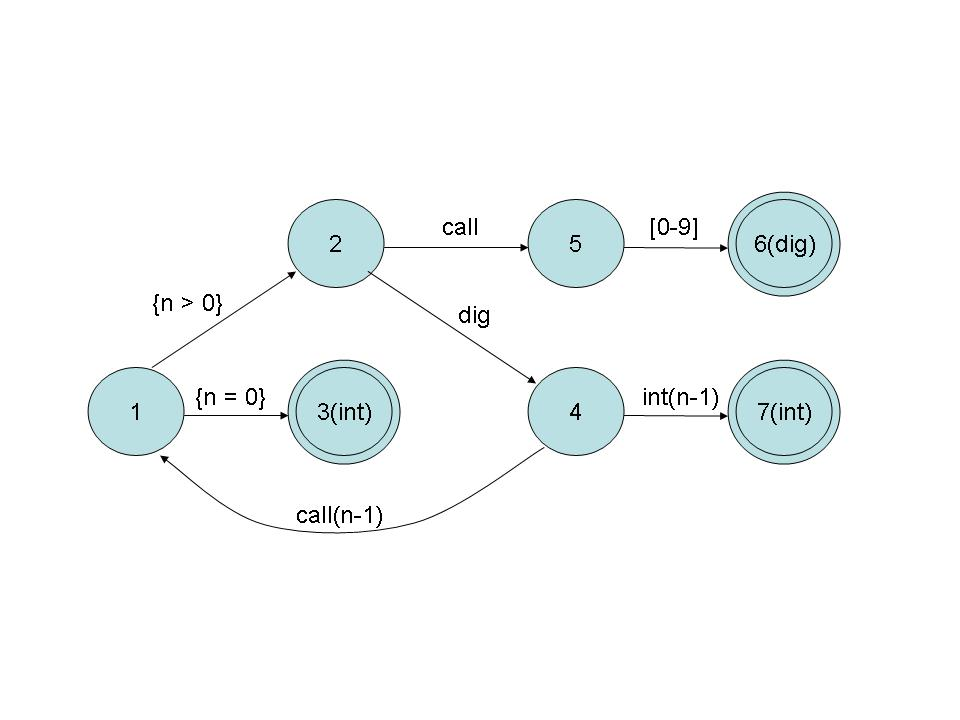
\includegraphics[width=100mm]{ddg-pic.jpg}
\end{center}
\vspace{-2cm}

\caption{Data Dependent Automaton for Parsing a Fixed-Width Integer 
with Width $n$.}
\label{fig:ddg-pic}
\end{figure}


Figure~\ref{fig:ddg-pic} gives a simple example of a data-dependent
automaton.    Such automata process inputs relative to environment
(in this case the environment involves a single variable $n$).
The automaton may follow edges between states marked
with a predicate $\{P\}$ when $P$ is true (edge 1-2 in Figure~\ref{fig:ddg-pic} is an example of this). 
Predicates such as $P$ may depend upon variables in the environment.
Call edges (such as edges 2-5 or 2-4 or 4-1) push the current state on to the stack
like a push-down automaton might do.  However, in addition to pushing a state, such
calls may be parameterized (as in the edge 4-1, which instantiates the
parameter $n$ with $n-1$).  Final states are denoted using double-circles.
These final states are also be marked by one or more grammar
non-terminal symbols ({\em e.g.,} state 6 is marked by non-terminal ``dig'').  
When control reaches a final state for non-terminal $A$, the execution
engine returns to the state on the top of the stack and follows
an edge marked by $A$.  For instance, upon arrival at state 6, 
control will return to state 2 (because that will have been placed
on the top of the stack by the call from 2 to 5) and then from there,
control will proceed along the edge marked ``dig'' to state 4.  Overall,
given an initial (dynamically defined) parameter $n$, this automaton 
will recognize $n$ digits.

We have developed a non-deterministic execution semantics 
for these automata as well as an algorithm based on Earley's 
parsing algorithm~\cite{Earley}.  However, there remain many theoretical
and algorithmic questions left to answer about them, including:
(1) How do we map \pads{} descriptions to data-dependent automata?
(2) What data structures do we use to ensure efficient parse tree 
generation? (3) Data dependent grammars may be ambiguous.  How do we specify and
resolve ambiguities during parsing?  How do we detect ambiguities in the
presence of constraints? (4) What algorithms do we use to determinize data-dependent automata? 
More generally, how do we optimize data-dependent automata?
(5) What is the theoretical complexity of parsing in this new model?
Empirically, how do they compare to backtracking algorithms on grammars
of interest? (6) Can we develop algorithms to answer (or approximate) 
questions of emptiness or
inclusion of grammars or automata?

\paragraph*{New Tool Generation.}
The \pads{} system is already capable of generating a number of data processing tools automatically
from \pads{} descriptions.  However, we are intent on developing several more.  In general, we
will be driven by application and domain needs when it comes to development of new tools.  However,
there are two tools in particular that we already recognize will have great value to many users,
independent of domain.  

First, we plan to develop a tool that when given a description, will
generate example data that matches the description.  The purpose of such a tool is to 
automatically generate test cases for data processing tools and systems.  This task is
more challenging than it may seem at first due to the fact that \pads{} contains variable 
binding and constraints over multiple variables.
Hence, a simple random walk over a \pads{} description will not always generate data that matches 
the description -- sometimes the constraints will fail.  Despite this difficulty, we believe we 
will be able to develop effective and efficient test case generation through the use of 
theorem provers such as Z3~\cite{z3}.  A second challenge in test data generation is finding
ways to generate test data that does not match the input description and yet is ``close
enough'' to the description to model realistic error cases and failure modes that may trigger
software bugs.

A second tool we plan to develop is a query engine for directory systems in which the directory
matches a given description.  For example, a common question implmenters of the Coral
distributed system (mentioned earlier in this section) have is what the Coral traffic looked
like on hosts 1-5, on the week of december 22nd.  To answer this query, it is necessary to first select
out subsets of files based on the names of files and directories, and then to dig in to those files
and extract the key bits of data asked for.  The task becomes particularly tricky and tedious
from an engineering point of view when there are massive numbers of files and directories that
must be processed.  Using the team's experience building PADX~\cite{fernandez+:padx}, a query
engine for single-document ad hoc data files, we plan to develop a new tool for applying such
queries to collections of documents.   Naturally, this research effort will build 
directly upon the language design for multi-level directories proposed earlier
in this section.

\paragraph*{Collaboration Plan.}  PI Walker and Senior Personnel Fisher have collaborated on
data processing research together for 4 years.  Their collaboration plan
involves having weekly 1-hour teleconferences during which research problems are discussed and 
an agenda for the following week is set.  In addition, they will meet in person for face-to-face
meetings as necessary and dictated by the research problems. This structure has served them well in the past
and will continue to do so in the future.  
%In addition, Walker and Fisher have jointly supervised
%a number of graduate and undergraduate students in the past.  Again, these activities will continue. 

\subsection{Broader Impacts}
\label{sec:impacts}

%If funded, this project will have two major broad impacts.

\paragraph*{Industrial and Governmental Impact}
Today�s most important industries and governmental services run on
information. As different companies, NGOs, and governmental groups
implement buy, sell and exchange data, they are invariably frustrated
by the time and expense it takes to extract information from the
low-level formats in which their data is represented. 
The new technology proposed here will help improve the productivity
of companies and industries that face such data processing problems.
More directly,
through the PI's ongoing collaboration with Kathleen Fisher,
Yitzhak Mandelbaum and Trevor Jim at AT\&T Research, he has access
to industrial data sets and information on concrete industrial data
processing problems.  Working with AT\&T Research, he will have the tools
and resources required to help solve real problems in server log processing, 
network system monitoring and billing fraud detection.  In summary,
the PI and his team have the opportunity, connections and ability to perform
significant technology transfer.

\paragraph*{Supporting Research in the Natural Sciences}
Part of our mission will be
to provide support for the data processing needs of biologists,
chemists and physicists at Princeton University.
In particular, we will meet with Princeton computational biologists
Mona Singh, Hillary Coller and Olga Troyanskaya and their students
to determine their data processing needs.  In particular, Troyanskaya
has several projects that involve assembling and integrating various
ad hoc data sources (such as the GO data format described earlier in
this proposal) so that other computational biologists may query
and analyze them.  With the insights we learn from these colleagues, 
we will produce PADS descriptions for important biological data
sources used by them and others and use the PADS compiler to 
generate data processing tools for them.
In addition to working directly with scientists at Princeton, we
will make all of our software tools 
available on the web so academics anywhere can use them.

\paragraph*{Undergraduate and Graduate Education}
Princeton University has a very active undergraduate research program.
Princeton students usually do at least one semester of
Junior Independent Work and one semester of Senior Independent Work. 
Many students also do a year-long
Junior and Senior Theses.  
%For the past two years, PI Walker has
%lead the Princeton Computer Science Department Independent Work Program.
We believe that PADS is an excellent
platform for undergraduate independent work and we plan to link
undergraduate independent work with our interdisciplinary effort to
produce tools for biologists.  
%% We have already recruited Mark Daly,
%% a Princeton Senior who is doing his undergraduate senior thesis
%% on a PADS user interface and automatic format inference.
%% We hope encourage other undergraduates to help us build
%% specific data processing tools for the biological data formats
%% used in Princeton's Genomics Institute.
This will introduce students both to interesting and novel
computer science research and also allow them to build useful
tools for biological applications.  
%% The PI has a proven track record
%% when it comes to advancing graduate and undergraduate education
%% as he has organized two summer schools (2004, 2005) on technology for
%% secure and reliable programming and mentored several undergraduates,
%% the latest of which, Rob Simmons, won the Princeton Computer Science Department
%% Senior Thesis Award.
In addition to working with undergraduates, PI Walker, with the help of
Senior Personnel Fisher, will continue to advise Ph.D. students
in this area.

\subsection{Comparison with Other Research}
\label{sec:related}

There are a number of different kinds of parser generation tools such as
Lex and Yacc, ANTLR~\cite{antlr}, DFDL~\cite{dfdl-proposal,dfdl-primer}
and parser 
combinators~\cite{burge:parser-combinators,hutton+:parser-combinators}.
All of these tools provide ways for programmers to program parsers.
However, \pads{} and the research proposed in this paper provide much
more than just a parser.  In addition to a parser, \pads{} descriptions 
automatically generate a set of type declarations for the data representations
generated by parsers as well as error management infrastructure and powerful tools
such as \xml{} converters, format translators and query engines.  None of these
auxiliary items are provided by standard parser generators.  In addition, this
proposal adds new capabilities for specifying and managing multi-level directories
full of data, novel language design ideas for generating the descriptions/grammars themselves, 
new more powerful grammatical theories (standard parser generates process the LR fragment 
of the context free grammars) and additional new tools.

%% The oldest tools for describing data formats are parser generators such as
%% Lex and Yacc.  While excellent for parsing programming languages, Lex and Yacc
%% are too heavyweight for parsing the simpler ad hoc data formats one
%% runs into in the sciences.   
%% Unlike PADS, whose syntax is based on types from the well-known C language,
%% the syntax of Lex and Yacc is somewhat foreign.  Perhaps more importantly,
%% users must write a lexer, write a
%% grammar, and construct the in-memory representations by hand.  In
%% addition, they only work for ASCII data, they do not easily
%% accommodate data-dependent parsing, and they do not provide auxiliary
%% services such as automatic XML conversion, stastical analysis and
%% others.  Some more modern parser generators such as ANTLR~\cite{antlr} alleviate
%% a few of these problems, but they still do not automatically generate auxiliary tools
%% useful in processing ad hoc data nor do they provide good support for generating
%% rich, well-typed in-memory representations (ANTLR's in-memory representations
%% are very limited when compared with PADS and the extensions we propose).

%% There are parallels between PADS types and some of the elements of parser
%% combinator libraries found in languages like
%% Haskell~\cite{burge:parser-combinators,hutton+:parser-combinators}. 
%% However, as with most other general-purpose parsing tools, one cannot
%% simply put together a collection of Haskell's parser combinators and
%% automatically generate domain-specific programs such as 
%% an XML converter or a query engine, for instance.   T 

A somewhat different class of languages includes
\textsc{ASN.1}~\cite{asn} and \textsc{ASDL}~\cite{asdl}. 
Both of these systems specify the {\em logical\/} in-memory representation of data
and then automatically generate a {\em physical\/} on-disk representation.
Although useful for many purposes, this technology does not help
process data that arrives in predetermined, ad hoc formats.
Another language in this category is the Hierarchical Data Format 5 
(HDF5)~\cite{hdf5}.  This file format allows users to store scientific
data, but it does not help users deal with legacy ad hoc formats like PADS does.

The networking community has developed a number of domain-specific
languages~\cite{sigcomm00,bfd,gpce02} for parsing and printing binary data, particularly packets
from common networking protocols such as \textsc{TCP/IP} and also
\java{} jar-files.  Like \pads{}, these languages have a type-directed
approach to describing ad hoc data and permit the user to define
semantic constraints.  In contrast to our work, these systems handle
only binary data and assume the data is error-free or halt parsing if
an error is detected.  These systems also lack any of the new features
discussed in this proposal.
%Parsing non-binary data poses additional
%challenges because of the need to handle delimiter values and to
%express richer termination conditions on sequences of data. These
%systems also focus exclusively on the parsing/printing problem,
%whereas we have leveraged the declarative nature of our data
%descriptions to build additional useful tools.  

%% Currently, the Global Grid Forum is working on a standard
%% data-format description language for describing ad hoc data formats,
%% called DFDL~\cite{dfdl-proposal,dfdl-primer}.  Like \pads{},
%% DFDL{} has a rich collection of base types and supports a variety of
%% ambient codings.  Unlike \pads{}, DFDL{} does not support semantic
%% constraints on types nor dependent types, \eg{}, it is not possible to
%% specify that the length of an array is determined by some previously parsed field in the
%% data.  Our practical experience indicates that many ad hoc formats,
%% particularly binary formats, absolutely require dependent types in their
%% specifications.  DFDL{} is an annotated subset of XML{} Schema, which means
%% that the XML{} view of the ad hoc data is implicit in a DFDL{}
%% description.  DFDL{} is still being specified, so no DFDL-aware
%% parsers or data analyzers exist yet.  

% There are probably hundreds of tools that one might use if their data were
% in \xml.  However, the point of PADS is to allow scientists whose data is {\em not}
% already in \xml to get work done, particularly when that data contains errors,
% as ad hoc data often does.  Since many processes, machines, programs and other devices
% currently output data and a whole most of

There are also a number of XML-based data processing tools.  For instance,
XSugar~\cite{brabrand+:xsugar2005} allows user to specify an alternative non-XML
syntax for XML languages using a context-free grammar.  This tool
automatically generates conversion between XML and non-XML 
syntax. However,
since the basis of interconversion is a context free grammar, unlike PADS,
formats that required dependency may not be expressed.
XDTM~\cite{zhao+:sigmod05,xdtm} uses XML Schema to describe the locations of a collection
of sources spread across a local file system or distributed
across a network of computers and consequently is related to some of the research elements
presented in this proposal.
However, XDTM has no means of specifying the contents of files.  
The METS schema~\cite{mets} is similar to XDTM as it describes 
metadata for objects in a digital library,
including a hierarchy such objects. 

%% Commercial database products provide support for
%% parsing data in external formats so the data can be imported into
%% their database systems, but they typically support a limited number of
%% formats, \eg{}, COBOL copybooks.  Also, no declarative description of the
%% original format is exposed to the user for their own use, and they
%% have fixed methods for coping with erroneous data.  For these reasons,
%% PADS is complementary to database systems.  We strongly believe that
%% in the future, commercial database systems could and should support a 
%% PADS-like description language that allows users to import information from
%% almost any format.  We hope that our research on PADS will make a broad
%% impact in this area.

%% On the theoretical front, the scientific community's understanding of type-based languages for data description
%% is much less mature.  To the best of our knowledge, our work on
%% the DDC is the first to provide a formal interpretation of dependent 
%% types as parsers and to study the properties of these parsers including error correctness and
%% type safety.  Regular expressions and context-free grammars, the basis for Lex and Yacc
%% have been well-studied, but they do not have dependency, a key feature necessary for expressing
%% constraints and parsing ad hoc scientific data.
%% {\em Parsing Expression Grammars} (PEGs),
%% studied in the early seventies~\cite{birman+:parsing}, revitalized more 
%% recently by Ford~\cite{ford:pegs} and implemented using
%% ``packrat parsing'' techniques~\cite{ford:packrat,grimm:packrat}, 
%% are somewhat more similar to PADS recursive descent parsers. However, PADS does
%% not use packrat parsing techniques as the space overhead is too high for
%% large scientific data sets.  Moreover, our multiple interpretations of types in the DDC
%% makes our theory substantially different from the theory of PEGs.

%\subsection{Old Related}
%\section{Related Work}
\label{sec:related}

\edcom{Small summary followed by reference to thesis.}



\subsection{Results from Prior NSF Support}
\label{sec:prior}

%David Walker has received
%several NSF grants for developing secure and reliable
%programming language and compiler infrastructure.


%\paragraph*{David Walker, PI} 
\emph{NSF CT: Well-typed Trustworthy Computing in the 
Presence of Transient Faults} (CNS 0627650; 2006-2010; PI).  
This grant involves the development
of language and compiler support for transient fault tolerance.  
One of the ground-breaking results of this work was the development of
type system for guaranteeing fault
tolerance~\cite{perry+:ftal}.  This result was the first of its kind
and as a result won the PLDI 2007 best paper award and
was nominated as an ACM SIGPLAN CACM highlight in 2008.  In addition, 
the PIs and co-PIs have written a number of
other papers on this topic~\cite{walker+:faulty-lambda,reis:07:ieeemicro,perry+:control-faults,meola+:faulty-logic}, developed compiler infrastructure that implements their
ideas, organized and taught at summer schools~\cite{summer06,summer07},
engaged in undergraduate research (with one of their undergraduate mentees,
Lester Mackey, winning the CRA outstanding undergraduate research award) and
graduated several Ph.D. students who have gone on to join the US
workforce.

\emph{SEIII: Automatic Tool Generation for Ad Hoc Scientific Data} (IIS 0612147; 2006-2010; PI) and
\emph{CSR-SMA: Language support for data-centric systems monitoring} 
(CNS 0615062; 2006-2009; PI)
In this work, Walker, together with colleagues Kathleen Fisher 
(AT\&T research) and Yitzhak Mandelbaum (former Princeton Ph.D. student
advised by Walker; now AT\&T research), developed a domain-specific 
language called PADS for describing data 
formats~\cite{padsproj,fisher+:popl06,mandelbaum+:pads-ml,fisher+:dirttoshovels}.
When given a description, the PADS compiler can generate a suite
of useful data processing tools including query engine, XML translator,
data validator, and statistical analyzer.  In addition, Walker and 
his colleagues have
developed algorithms for learning the descriptions themselves automatically
from example data.  The many papers written during the course of this
research may be accessed on line as can software the PI and his colleagues
have developed~\cite{padsweb,padsdemo}.  Again, both Ph.D. students
and undergraduates have participated in these research efforts.
The current proposal builds upon the infrastructure
and scientific ideas developed in this previous work.

%%%%

\emph{CAREER: Programming
Languages for Secure and Reliable Component Software Systems}
(NSF CCR-0238328; 2003-2008; PI)
and 
\emph{Collaborative Research: High-Assurance Common Language Runtime} 
(NSF CCR-0208601; 2002-2007; Co-PI) and
\emph{Collaborative Research: CSR-PDOS:Managing OS Extensibilty via 
Aspect-oriented Programming Technology} (NSF CSR 0615213; 2006-2009; Co-PI).
The
goal of these awards was to develop new programming language
technology that will improve the security and reliability of component
software systems.  More specifically, Walker and his students developed 
a new theory of security monitors as formal automata that transform
untrusted applications as they 
execute~\cite{ligatti+:edit-automata,ligatti+:renewal}.  This
formal model allowed them to prove a variety of important theorems
concerning the power of different enforcement mechanisms
as well as serving as the underpinnings for several novel
language design ideas revolving around safe aspect-oriented programming
language technologies~\cite{bauer+:polymer,walker+:aspects,dantas+:harmless-advice,dantas+:harmless-popl}.  As part of his efforts to develop more reliable
software, Walker also worked extensively on the
development of type systems, program logics and
type-directed and certifying compilation~\cite{ahmed+:stack,ahmed+:hierarchical-storage,jia+:ilc,walker:attapl}.  Once again, in addition to publishing
papers, Walker created software, graduated two Ph.D. students,
mentored undergraduate research, and shared his knowledge by teaching 
at summer schools for graduate students.

%Walker's grants in this area also allowed him to be a leader in programming
%languages and security education. In 2004 and 2005 he organized a
%10-day summer school on software security and reliable computing,
%attended by over 100 participants
%combined~\cite{summerschool04,summerschool05}.  Also in 2005, his
%undergraduate research advisee, Rob Simmons, won the Princeton
%Computer Science Department Senior Thesis Award.  He also dedicated time
%to writing a chapter of a new textbook on typed programming
%languages~\cite{walker:attapl}.

%% \paragraph*{David Walker, PI}
%% (CCR 0238328; CAREER: Programming Languages for Secure and Reliable 
%% Component Software Systems)
%% The goal of Walker's career award is to develop new programming language
%% technology that will improve the security and reliability of component software systems.
%% More specifically, Walker and his students have begun to develop new techniques for defining,
%% implementing and reasoning about run-time enforcement of program properties.
%% For example, he developed a rich new theory of security monitors as formal
%% automata that transform untrusted program behavior as they 
%% execute~\cite{ligatti+:edit-automata}.
%% This theory allows security
%% architects to model a variety of different sorts of run-time
%% enforcement mechanisms, to prove that certain mechanisms can or cannot
%% enforce various security properties, and to compare the power of
%% different classes of security monitors.    Recently, Walker 
%% has used the theory to prove the surprising new result that powerful run-time
%% program monitors can enforce certain kinds of liveness properties~\cite{ligatti+:renewal}
%% and build an implementation for Java~\cite{bauer+:polymer}.

%% Walker's security monitoring language is a form of aspect-oriented programming language.
%% In order to better understand aspect-oriented technologies and their
%% potential impact on security, Walker formalized and proved
%% safe the {\em first} higher-order, strongly-typed calculus of 
%% aspects~\cite{walker+:aspects}, built an implementation and extended it with facilities for polymorphic
%% and type-directed programming~\cite{dantas+:polyaml}.  This calculus defines
%% both static typing rules and the execution behavior of aspect-oriented
%% programs.  Consequently, it may
%% serve as a starting point for analysis of deeper properties of programs.
%% Recently, he has used the calculus to study the design of a
%% program analysis that determines the effect of security monitors on
%% the code they monitor~\cite{dantas+:harmless-advice,dantas+:harmless-popl}.   The analysis
%% can guarantee that a security monitor does not interfere with the 
%% original application, which greatly increases a user's incentive
%% to apply security patches.

%% To complement his work on run-time monitoring programs, Walker has also
%% developed several type systems to ensure basic type and memory safety conditions
%% for low-level programs.  Basic type- and memory-safety guarantees provide a foundation on which
%% richer security mechanisms can be implemented.  More specifically, he
%% has extended his earlier work on typed assembly language (TAL)~\cite{morrisett+:tal,morrisett+:journal-stal} with
%% logic-based type systems that can detect memory errors involving
%% stack-allocated data~\cite{ahmed+:stack,jia+:stack} and heap or region-allocated
%% data~\cite{ahmed+:hierarchical-storage}.  In addition to studying memory safety
%% properties, Walker has shown how to use related type-theoretic and logical techniques
%% to verify programs~\cite{jia+:ilc} and enforce general software
%% protocols~\cite{mandelbaum+:refinements}.  

%% Finally, Walker's career grant allowed him to be a leader in
%% programming languages and security education. In 2004 and 2005 he organized
%% a 10-day summer school on software security and reliable computing,
%% attended by over 100 participants combined~\cite{summerschool04,summerschool05}.  He has also written a
%% chapter of a new textbook on type systems~\cite{walker:attapl}.  Also in 2005, his
%% undergraduate research advisee, Rob Simmons, won the Princeton Computer Science Department
%% Senior Thesis Award.



\newpage
%%%%%%%%%%%%%%%%%%%%%%%%%%%%%%%%%%%%%%%%%%%%%%%%%%%%%%%%%%%%%%%%%%%%%%%%%%%%
\section{References Cited}

{\bibliographystyle{abbrv}
\bibliography{pads-long,pads,galax,padsdave}
}
%{\bibliographystyle{abbrv}
% \small\bibliography{pads}
%} 
\newpage
%%%%%%%%%%%%%%%%%%%%%%%%%%%%%%%%%%%%%%%%%%%%%%%%%%%%%%%%%%%%%%%%%%%%%%%%%%%%
%\section{Biographical Sketch}
%\documentclass[11pt]{article}
        % Use font 11pt Roman.
%\documentstyle{article}

\usepackage{url}

%\def\references{\newpage\section*{References}}
%\newcounter{refcount}
%\def\lit#1{~[\ref{#1}]}
%\def\cit#1#2#3#4{#1\quad#2\quad{\it #3}\quad #4\vskip.15in }
%\def\citb#1#2#3{#1\quad{\it #2}.\quad#3.}
%\def\citu#1#2{#1\quad#2.}


\newcommand{\comment}[1]{}


% No header or foot; top 2.0in, left 0.6in, right 0.9in, bottom 0.5in

%\pagestyle{empty}
%\topmargin=-.5in
%\textheight=8.8in
%\leftmargin=-1.0in
%\oddsidemargin=.25in
%\oddsidemargin=.25in
%\textwidth=6.2in

\setlength{\textheight}{22.8true cm}
%\setlength{\textwidth}{15.4true cm}
\setlength{\textwidth}{15.9true cm}
\setlength{\oddsidemargin}{.55true cm}
\setlength{\evensidemargin}{.55true cm}
\setlength{\topmargin}{-1.0cm}
\pagestyle{empty}

\newlength{\oldparindent}
\setlength{\oldparindent}{\parindent}
\setlength{\parindent}{0pt}

% No indentation at the beginning of paragraphs.

% Don't hyphenate.
%\hyphenpenalty=10000


% Rsection: a resume section environment.
\newenvironment{Rsection}[1]{
  \noindent{\bf #1}
  \begin{list}{}{\topsep=-\parskip
                 \leftmargin=-0.0in}
    \item[]
}{
  \end{list}
%  \vspace \baselineskip
}
                           
% Section: a resume section environment.
\newenvironment{Section}[1]{
  \centerline{\bf #1}
  \begin{list}{}{\topsep=-\parskip
                 \leftmargin=-0.5in}
    \item[]
}{
  \end{list}
%  \vspace \baselineskip
}

% edlist: a resume education list environment.
\newenvironment{edlist}{
  \begin{list}{}{\topsep=-\parskip
                 \itemsep=0.5\baselineskip
                 \leftmargin=0.25in}
}{
  \end{list}
}


% edlist2: a resume education list environment.
\newenvironment{edlist2}{
  \begin{list}{}{\topsep=-\parskip
                 \itemsep=0.5\baselineskip
                 \leftmargin=0.25in
                 \setlength{\rightmargin}{\leftmargin}
                 \textwidth=4in}
}{
  \end{list}
}
                           

% honorlist: a resume honor list environment.
\newenvironment{honor2list}{
  \begin{list}{}{\topsep=-\parskip
                 \itemindent=-0.in
                 \itemsep=0.0\baselineskip
                 \leftmargin=.25in}
}{
  \end{list}
}  

\newenvironment{honor2enum}{
  \begin{enumerate}{}{\topsep=-\parskip
                 \itemindent=-0.in
                 \itemsep=0.0\baselineskip
                 \leftmargin=.25in}
}{
  \end{enumerate}
}  

\newenvironment{honor3enum}{
  \begin{enumerate}{}{\topsep=-\parskip
                 \itemindent=-0in
                 \itemsep=0.0\baselineskip
                 \leftmargin=.25in}
}{
  \end{enumerate}
}  



% honorlist: a resume honor list environment.
\newenvironment{honorlist}{
  \begin{list}{}{\topsep=-\parskip
                 \itemindent=-0.in
                 \itemsep=0.2\baselineskip
                 \leftmargin=.25in}
}{
  \end{list}
}  


% joblist: a resume job list environment.
\newenvironment{joblist}{
  \begin{list}{}{\topsep=-\parskip
                 \itemsep=0.5\baselineskip
                 \leftmargin=0.5in}
}{
  \end{list}
}

                                      
% job: a job entry for a joblist environment
\newcommand{\job}[3]{
  \item[]
  \begin{tabbing}
    \hspace{-0.5in}\=\hspace{1.5in}\=\kill
    \>    {\it #1:}       \> #2   \\
    \>                    \> #3   \\
  \end{tabbing}
  \vspace{-\baselineskip}
}

              
%%%%%%%%%%%%%%%%%%%%%%%%%%%%%%%%%%%%%%%%%%%%%%%%%%%%%%%%%%%%%%%%%%%%%%%%%%%%%%%




%%%%%%%%%%%%%%%%%%%%%%%%%%%%%%%%%%%%%%%%%%%%%%%%%%%%%%%%%%%%%%%%%

%\leftmargin=-1in
\begin{document}


\centerline{\Large \bf {\LARGE \bf D}AVID {\LARGE \bf W}ALKER}
\vskip .3in

\normalsize
\it
\begin{tabular}{@{\hspace{0in}}l@{\hspace{1.4in}}l}
35 Olden Street   & Phone: (609) 258--7654  \\
Princeton University   & Email: {\rm dpw@cs.princeton.edu} \\
Princeton, NJ 08544

\end{tabular}
\rm
\vskip.3in

\begin{Rsection}{\Large \bf {Professional Preparation}}
\vskip.1in
\begin{edlist}

\item {\bf Queens University, Kingston, Ontario, Canada }
  \begin{honor2list}
  \item {Computer Science, B.Sc. Honors, 1995.}  

  \end{honor2list}
\item {\bf Cornell University}
\begin{honor2list}
\item {Computer Science, M.S. 1999.}
\item {Computer Science, Ph.D. 2001.}
\end{honor2list}
\end{edlist}
\end{Rsection}


\vskip.3in
\begin{Rsection}{\Large \bf {Appointments}}
\vskip.1in
\begin{edlist}
\item {\bf Princeton University}\\
{\bf  Department of Computer Science} \\
%\vskip .05in
\vspace{-1ex}
\begin{honor2list}
\item Assistant Professor, Feb. 2002--present.
\end{honor2list}

\item {\bf Carnegie Mellon University}\\
{\bf  Department of Computer Science} \\ 
%\vskip .05in
\vspace{-1ex}
\begin{honor2list}
\item Postdoctoral Fellow, Oct. 2000--Oct. 2001
\end{honor2list}


%\newpage
\end{edlist}
\end{Rsection}


\vskip.3in
\begin{Rsection}{{\Large \bf {Selected Publications}} 
}
\vskip.1in
\begin{edlist}

\item {\bf Selected papers of greatest relevance (in chronological order)}
\begin{honor2enum}
\vskip .1in

\item The Next 700 Data Description Languages. Kathleen Fisher, 
Yitzhak Mandelbaum and David Walker.  ACM SIGPLAN-SIGACT Symposium 
on Principles of Programming languages.  To appear, January 2006.
Available at \url{http://www.cs.princeton.edu/~dpw/papers.html}

\item LaunchPADS: A System for Processing Ad Hoc Data. Mark Daly, 
Mary Fernandez, Kathleen Fisher, Yitzhak Mandelbaum and David Walker.  
Demo Paper in PLAN-X 06:  Programming Language Technologies for XML.  
To appear, January 2006.
Available at \url{http://www.cs.princeton.edu/~dpw/papers.html}. 

\item Dynamic Typing with Dependent Types (extended abstract).
Xinming Ou, Gang Tan, Yitzhak Mandelbaum, and David Walker.  In the
3rd IFIP International Conference on Theoretical Computer Science,
August, 2004.

\item 
A Type-Theoretic Interpretation of Pointcuts and Advice.  
Jay Ligatti, David Walker and Steve Zdancewic.  
In the ACM SIGPLAN International 
Conference on Functional Programming, August 2003.

\item An Effective Theory of Type Refinements.  Yitzhak Mandelbaum, 
David Walker and Robert Harper.  In the ACM SIGPLAN International 
Conference on Functional Programming, August 2003. 


%


\end{honor2enum}

\newpage
\item {\bf Selected other publications (in chronological order):}
\begin{honor2enum}

\item Harmless Advice.  Daniel S. Dantas and David Walker.  
ACM SIGPLAN-SIGACT Symposium on Principles of Programming Languages.  
To appear, January 2006. 
Available at \url{http://www.cs.princeton.edu/~dpw/papers.html}

\item Composing Security Policies in Polymer.  
Lujo Bauer, Jarred Ligatti and David Walker.
ACM SIGPLAN Conference on Programming Language Design and 
Implementation.  June 2005.

\item Substructural Type Systems.  David Walker.
Chapter 1 of Benjamin Pierce, ed.,
Advanced Topics in Type Systems for Programming Languages.  
MIT Press, January 2005.

\item 
Typed Memory Management via Static Capabilities. 
David Walker, Karl Crary, and Greg Morrisett. ACM Transactions on Programming Languages and
Systems, 22(4):701-771, July 2000.  

\item 
From System F
to Typed Assembly Language. 
Greg Morrisett, David Walker, Karl Crary, and Neal Glew. 
ACM Transactions on Programming Languages
and Systems, 21(3):528-569, May 1999.


\end{honor2enum}

\end{edlist}
\end{Rsection}



\vskip.3in
\begin{Rsection}{\Large \bf {Synergistic Activities}}
\begin{honor2list}
\vskip .1in
\begin{itemize}
\item Emerson Junior Faculty Award for excellence in
research and teaching.  (Princeton Award) May 2005.
\item Alfred P. Sloan Fellow.  Sept 2004-Sept 2006. 
\item Summer School on Reliable Computing.  Program
Co-Chair and Organizer.  July 2005.  Supported by NSF.
A 10-day summer school on type systems, program analysis,
software model checking, and domain specific languages
aimed at teaching the latest research on improving software reliability. 
\item Summer School on Software Security: Theory to Practice.  Program
Co-Chair and Organizer.  
June 2004.  Supported by ACM SIGPLAN, NSF, and Microsoft.
A 10-day summer school that taught the fundamentals of
software security.  
\item 
Program Chair for FOAL 2005, SPACE 2006.  Program committee
for ICFP 2004, TLDI 2005, FOAL 2006, ICALP 2006, POPL 2007.  
Periodic program chair and host for
the New Jersey Programming Languages Seminar, 2002-now.
\item Publicity chair for ACM SIGPLAN-SIGACT Symposium on
Principles of Programming Languages, 2003--2006.
\end{itemize}



\end{honor2list}
\end{Rsection}
\vskip.3in
\begin{Rsection}{\Large \bf {Collaborators and Other Affiliations}}
\begin{itemize}
\vskip .1in
\item Collaborators: 
Amal Ahmed (Harvard),
Andrew Appel (Princeton),
Zena Ariola (U of Oregon),
Lujo Bauer (Carnegie Mellon),
Iliano Cervesato (Tulane),
%Karl Crary (Carnegie Mellon University),
%Daniel Dantas (Princeton University),
%Ed Felten (Princeton University),
Mary Fernandez (AT\&T),
Kathleen Fisher (AT\&T),
Neal Glew (Intel),
Daniel Grossman (U of Washington),
Robert Harper (Carnegie Mellon),
%Limin Jia (Princeton University),
%Jarred Ligatti (Princeton University),
%Yitzhak Mandelbaum (Princeton University),
Greg Morrisett (Harvard),
Benjamin Pierce (U of Pennsylvania),
Frank Pfenning (Carnegie Mellon),
%Fred Smith (MathWorks),
%Frances Spalding (Princeton),
%Daniel Wang (Princeton),
Geoffrey Washburn (U of Pennsylvania),
Kevin Watkins (Carnegie Mellon),
Stephanie Weirich (U of Pennsylvania),
Steve Zdancewic (U of Pennsylvania)

\item Graduate (Ph.D.) Advisor: 
Greg Morrisett (Cornell University, now Harvard University)
\item Thesis Advisees (graduated): none
\item Thesis Advisees (current): Dan Dantas, Limin Jia, Jarred Ligatti, 
Yitzhak Mandelbaum, Frances Spalding
\end{itemize}
\end{Rsection}



% \iffalse
% \vskip.3in
% \begin{Rsection}{\Large \bf {Selected Awards and Fellowships}}
% \begin{itemize}
% \vskip .1in
% \end{itemize}
% \end{Rsection}
% \fi




%\newpage

%\newpage





%%%%%$$^{\ref{fn:second}}$







%\vskip.3in




\end{document}



%They are in separate files now (see cv/lastname-cv.tex).

%%%%%%%%%%%%%%%%%%%%%%%%%%%%%%%%%%%%%%%%%%%%%%%%%%%%%%%%%%%%%%%%%%%%%%%%%%%%
%\section{Budget}

%The budget pages (no longer necessary because of fastlane). 

%%%%%%%%%%%%%%%%%%%%%%%%%%%%%%%%%%%%%%%%%%%%%%%%%%%%%%%%%%%%%%%%%%%%%%%%%%%%
%\section{Current and Pending Support (NSF Form 1239)}

%The current-and-pending pages (no longer necessary because of fastlane). 

%%%%%%%%%%%%%%%%%%%%%%%%%%%%%%%%%%%%%%%%%%%%%%%%%%%%%%%%%%%%%%%%%%%%%%%%%%%%
%\section{Facilities, Equipment and Other Resources (NSF Form 1363)}

%The facility page (no longer necessary because of fastlane).

%%%%%%%%%%%%%%%%%%%%%%%%%%%%%%%%%%%%%%%%%%%%%%%%%%%%%%%%%%%%%%%%%%%%%%%%%%%%
%\section{Special Information and Supplementary Documentation}

%We may consider asking AT\&{}T to provide a support letter.

\end{document}


